\chapter{Evaluation} \label{chap:Evaluation}
The evaluation of this work has two objectives. First, to make sure that the modified designs still produce correct output. Meaning that the result of an operation when decrypted is the same for both the modified and unmodified versions of the library. Secondly, to profile each design and compare run times of the modified libraries to the unmodified library. These time comparisons will occur at multiple levels to best understand each design, and how they compare to the serial version.

Distributed systems achieve the best efficiency when working on large inputs, not small ones. This is because there is some overhead associated with setting up and distributing work. For GPU designs, this overhead time happens when transferring the data to and from the GPU. For distributed computing designs, the overhead time is also in the memory transfers like the GPU, but instead of transferring to the GPU, the memory transfers are between machines. This overhead costs time, that when working with small inputs, usually takes even longer than the operation to complete. Thus the distributed design causes a run time slow down compared to the serial version for small input sizes. However, when working with large amounts of data, the time saved to complete the operation is so great, that the overhead costs are worth it. This characterization of distributed systems is prevalent for these designs, which will be seen later. For these encryption systems, large input sizes occur when $size\_of\_row$ is large. For any distributed system, large has a variable meaning that is relative to the system being examined. It could be anywhere from a few hundred thousand to a few billion. For these libraries, large is defined to be above a few hundred thousand. As discussed in the design chapters, $size\_of\_row$ is the length of the vectors in \verb|map|. To best demonstrate the effect $size\_of\_row$ has on the system, $size\_of\_row$ is steadily increased during the testing, so its effect on each design can be seen and compared to the original design.

To evaluate these designs a few profiling tools were used, discussed in Section \ref{sec:EvaluationTools}. The test environments used for each design are detailed in Section \ref{sec:TestingEnvironment}. The results for GPUHElib are examined in Section \ref{sec:GPUHElibEvaluationResults}, followed by the results for DistributedHElib in Section \ref{sec:DistributedHElibEvaluationResults}. Finally some conclusions are drawn regrading both of these designs in Section \ref{sec:EvaluationConclusions}

\section{Evaluation Tools} \label{sec:EvaluationTools}
The following tools were used to evaluate the correctness of the modified libraries and record run times at various levels in the library.

\subsection{Test Program}
A test program was created based on testing programs provided with the original unmodified version of HElib. This new test program first sets up the ciphertexts that are used during computation. Two ciphertexts are created, both are the integers, $0$ to $ num\_slots\_in\_plaintext$. 

Three operations are reported on in this document, of the six implemented. They are addition, subtraction, and multiplication of one ciphertext with another ciphertext. The other three operations supported, addition, subtraction, and multiplication of a ciphertext and a number, were not reported, as preliminary tests showed that they displayed similar results to their ciphertext-only counterparts. It was decided that for conciseness and to avoid repetition, that they would be left out of this document.

The program requires that the user pass in the $size\_of\_row$ they would like to use, which as discussed above, will be incremented during testing. The test program then performs each operation, checking the decrypted result after each operation to make sure that the results are correct, before moving on. Timing blocks were placed around each operation to record the overall time it took to perform the operation. The timers were printed out after each operation. Lower level timers, discussed below, were reset after each operation, so the lower level times reported with each operation were only times recorded for that operation.

This test program was compiled twice for both designs, first linking against the unmodified library, and second against the modified library. This produced two executables, that were then run to generate the results described below.

\subsection{HElib Timing Functions}
The standard version of HElib provides fine grained timing functions that can be placed anywhere throughout the library. To utilize these functions is simple. First a timer is created. Upon the creation of the timer, it is started. A call to \verb|stop| is made in code when the timer should stop. A timer can be started and stopped multiple times, and the average time will be recorded. The timers are stored in a map, and can be reset if needed. This setup allows for fine grained measurement of functions and detailed profiling of run times. 

Each design, serial HElib, GPUHElib, and DistributedHElib required the timers be placed at some similar places, for comparison purposes, and some distinct places, in order to assess the efficiency of each unique design.

\subsubsection{Serial HElib Timer Placement}
There were two levels at which timers were placed, with each successive level more fine grained. The first level was in the test program, described above. This is the circuit level. The other timer was placed at the function level, inside the function that performed the operations in \verb|DoubleCRT|. This function was where the double \verb|for| loop was located that both of the distributed designs are trying to improve upon.

\subsubsection{GPUHElib Timer Placement}
For GPUHElib, there are three levels at which timers were placed. As described above, the first timer was placed at the circuit level in the test program. This records the time that the entire operation took. The second level of timing was the function level. At this level a timer was placed in the function that is performing the operations in \verb|DoubleCRT|. These first two timer levels allow for comparison against the serial version, as the serial version also has timers placed at these levels. The third and lowest level is the phase level. Four timers are placed at this level to record the setup (vector and stream creation), phase one (host to device memory transfer), phase two (GPU computation), and phase three (device to host memory transfer) times. The timers at this level allow for the times gathered at level two to be broken down even further, and allow each phase of level two to be examined closer.

\subsubsection{DistributedHElib Timer Placement}
For DistributedHElib, there are three levels at which timers were placed. The first at the circuit level in the test program. The second at the function level, in \verb|DoubleCRT|, where the operation is being performed. These first two timer levels are necessary for the comparison against the serial version, as the serial version also has timers at these two levels. The third consists of two timers: the distribute (where the job assignment and data partitioning happens) and the wait (where the sync function is called, and the dispatcher node is waiting for the compute nodes to finish and send back their results). This third level allows for a breakdown of the function level for further analysis. 

\section{Testing Environment} \label{sec:TestingEnvironment}
Both systems required unique testing environments that had the capabilities needed for each design. Both variants used machines with 64-bit Intel Core 2 Duo CPUs running at 3.0 Ghz with about 4 Gb of DDR2, 800 Mhz RAM.

\subsection{GPU Testing Environment}
GPUHElib was tested on a machine with a NVIDIA Quadro NVS 290 GPU, which has 256 MB of RAM. Also this particular GPU only has one copy engine. Thus the tests reported here are using the 2-Way Pipelining design discussed in Section \ref{sec:Pipelining}. CUDA version 6.5 was used.

\subsection{Distributed Computing Testing Environment}
DistributedHElib was tested on a cluster of machines all connected through Ethernet. OpenMPI version 1.8.5 was used. Three cluster configurations were used, one with 4 nodes, one with 8 nodes, and one with 16 nodes.

\section{GPUHElib Evaluation Results} \label{sec:GPUHElibEvaluationResults}
As discussed earlier in this chapter, GPUHElib has three levels of timing information begin recorded. The first, and highest level, is the circuit level, where the high level operation is being computed. The second level is the function level, inside \verb|DoubleCRT| where the \verb|parts| are being operated on. And the lowest level is the phase level, where timing results are recorded for all four phases of the operation. The timing results for each of these levels is discussed in more detail in the following sections.

\subsection{GPUHElib Circuit Level Run Times}
\begin{table}[p]
\centering
\begin{tabular}{ | r | r | r | r | r | r | r | }
 \multicolumn{1}{ r }{} & \multicolumn{6}{ c }{$size\_of\_row$} \\ \cline{2-7}
 \multicolumn{1}{ r |}{} & $1{,}000$ & $10{,}000$ & $100{,}000$ & $200{,}000$ & $300{,}000$ & $400{,}000$ \\ \hline
 Add & 1.400E-05 & 1.080E-04 & 2.545E-03 & 5.396E-03 & 5.354E-03 & 1.053E-02 \\ \hline
 Sub & 1.400E-05 & 1.300E-04 & 2.532E-03 & 5.304E-03 & 5.366E-03 & 1.075E-02 \\ \hline
 Mul & 4.962E-03 & 1.036E-01 & 1.157 & 2.648 & 7.217 & 1.232E+01 \\ \hline
\end{tabular}
\caption{Serial HElib circuit level run times (in seconds)}
\label{tab:GPUserialLevel1Runtimes}
\end{table}

\begin{table}[p]
\centering
\begin{tabular}{ | r | r | r | r | r | r | r | }
 \multicolumn{1}{ r }{} & \multicolumn{6}{ c }{$size\_of\_row$} \\ \cline{2-7}
 \multicolumn{1}{ r |}{} & $1{,}000$ & $10{,}000$ & $100{,}000$ & $200{,}000$ & $300{,}000$ & $400{,}000$ \\ \hline
 Add & 1.050E-03 & 1.675E-03 & 8.972E-03 & 1.646E-02 & 1.671E-02 & 3.704E-02 \\ \hline
 Sub & 1.012E-03 & 1.805E-03 & 9.023E-03 & 1.683E-02 & 1.682E-02 & 3.700E-02 \\ \hline
 Mul & 1.106E-02 & 1.187E-01 & 1.309 & 2.868 & 7.393 & 9.333 \\ \hline
\end{tabular}
\caption{GPUHElib circuit level run times (in seconds)}
\label{tab:GPULevel1Runtimes}
\end{table}

\begin{figure}[p]
\centering

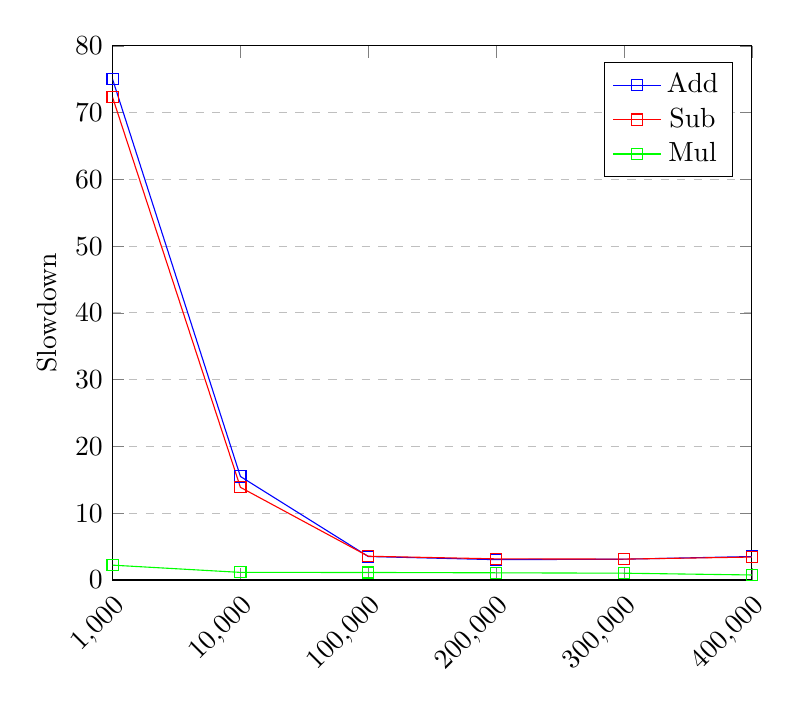
\begin{tikzpicture}
\begin{axis}
[
    ylabel={Slowdown},
    width=.8\textwidth,
    xmin=1, xmax=6,
    ymin=0, ymax=80,
    xtick={1,2,3,4,5,6},
    xticklabels={$1{,}000$, $10{,}000$, $100{,}000$, $200{,}000$, $300{,}000$, $400{,}000$},
    ytick={80,70,60,50,40,30,20,10,0},
    legend pos=north east,
    ymajorgrids=true,
    grid style=dashed,
    x tick label style={rotate=45,anchor=north east},
]

\addplot[color=blue,mark=square]
    coordinates {
    (1,75)(2,15.50925926)(3,3.525343811)(4,3.049481097)(5,3.121404557)(6,3.519144893) };
    
\addplot[color=red,mark=square]
    coordinates {
    (1,72.28571429)(2,13.88461538)(3,3.563586098)(4,3.172511312)(5,3.1339918)(6,3.441354293) };

\addplot[color=green,mark=square]
    coordinates {
    (1,2.229544538)(2,1.146005137)(3,1.131587363)(4,1.083041024)(5,1.024489643)(6,0.757830934) };
    
\legend{Add,Sub,Mul}
 
\end{axis}
\end{tikzpicture}

\caption{Run Time Comparison at Circuit Level}
\label{fig:level1ComparisonSerialGPU}
\end{figure}

Table \ref{tab:GPUserialLevel1Runtimes} and Table \ref{tab:GPULevel1Runtimes} display the run times for serial HElib and GPUHElib tests respectively. Both tests were run with inputs sizes starting at 1,000 and increasing until 400,000. 

Figure \ref{fig:level1ComparisonSerialGPU} visualizes these times as the slowdown of GPUHElib over serial HElib. A value of 1 means that the serial version and the GPU version had the same run time. Above 1 means that the GPU design has a slower run time, and below 1 means that the GPU has a faster run time.

One can see in Figure \ref{fig:level1ComparisonSerialGPU} that for the smaller input sizes, the run times for the GPU are much larger than the serial version for addition and subtraction. They started off taking about 72 times as long to complete, compared to the serial version. The multiplication operation also starts off taking longer, however only about 2.2 times as long. The run times for serial HElib and GPUHElib get closer and closer, as the inputs sizes approach 400,000. The addition and subtraction circuit run times minimize at about 3 times as long, for the 300,000 size input. However for the 400,000 size input, the times go in the opposite direction desired, becoming about 3.5 times as long. The multiplication circuit actually has the best results, with the 400,000 test taking about .75 times the serial version. The multiplication circuit took about 3/4 the time to complete in GPUHElib compared to the serial version. While this result might look good, further analysis of the lower level tests show that this was probably not caused by the usage of the GPU, but by other operations computed during the multiplication operation being faster. The function level run times will be examined next.

\subsection{GPUHElib Function Level Run Times}
\begin{table}[p]
\centering
\begin{tabular}{ | r | r | r | r | r | r | r | }
 \multicolumn{1}{ r }{} & \multicolumn{6}{ c }{$size\_of\_row$} \\ \cline{2-7}
 \multicolumn{1}{ r |}{} & $1{,}000$ & $10{,}000$ & $100{,}000$ & $200{,}000$ & $300{,}000$ & $400{,}000$ \\ \hline
 Add & 5.000E-06 & 4.825E-05 & 1.007E-03 & 2.648E-03 & 2.653E-03 & 5.466E-03 \\ \hline
 Sub & 5.000E-06 & 6.150E-05 & 1.259E-03 & 2.644E-03 & 2.674E-03 & 5.366E-03 \\ \hline
 Mul & 2.900E-05 & 2.830E-04 & 2.879E-03 & 5.863E-03 & 5.856E-03 & 1.176E-02 \\ \hline
\end{tabular}
\caption{Serial HElib function level run times (in seconds)}
\label{tab:GPUserialLevel2Runtimes}
\end{table}

\begin{table}[p]
\centering
\begin{tabular}{ | r | r | r | r | r | r | r | }
 \multicolumn{1}{ r }{} & \multicolumn{6}{ c }{$size\_of\_row$} \\ \cline{2-7}
 \multicolumn{1}{ r |}{} & $1{,}000$ & $10{,}000$ & $100{,}000$ & $200{,}000$ & $300{,}000$ & $400{,}000$ \\ \hline
 Add & 5.210E-04 & 8.298E-04 & 4.392E-03 & 8.257E-03 & 8.346E-03 & 1.864E-02 \\ \hline
 Sub & 5.020E-04 & 8.950E-04 & 4.498E-03 & 8.398E-03 & 8.395E-03 & 1.848E-02 \\ \hline
 Mul & 5.302E-04 & 1.006E-03 & 6.599E-03 & 1.273E-02 & 1.276E-02 & 2.687E-02 \\ \hline
\end{tabular}
\caption{GPUHElib function level run times (in seconds)}
\label{tab:GPULevel2Runtimes}
\end{table}

\begin{figure}[p]
\centering
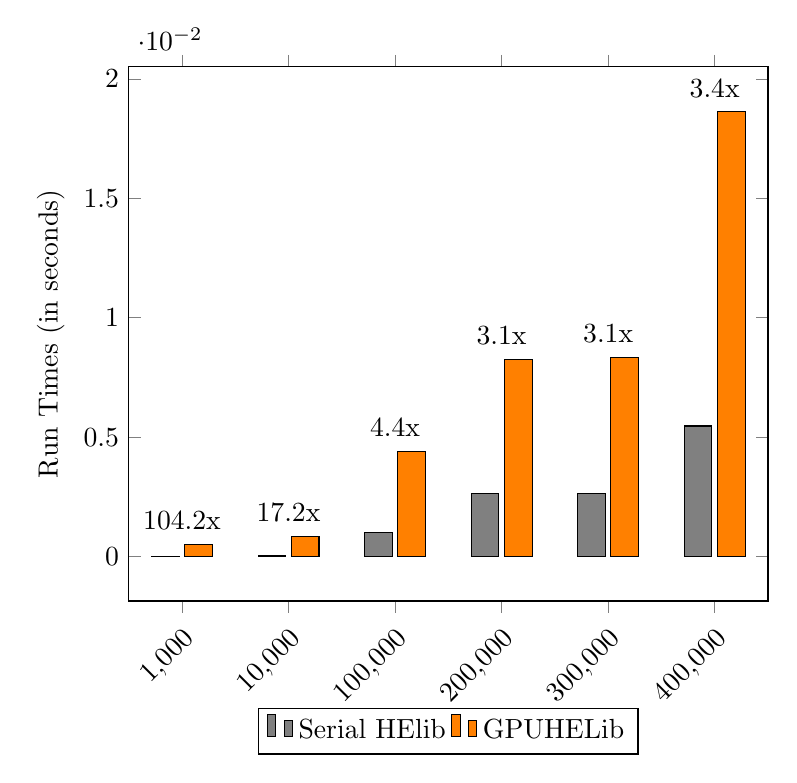
\begin{tikzpicture}

\begin{axis}[
    ybar,
    width=.8\textwidth,
    legend style={at={(0.5,-0.2)},anchor=north,legend columns=-1},
    ylabel=Run Times (in seconds),
    symbolic x coords={$1{,}000$,$10{,}000$,$100{,}000$,$200{,}000$,$300{,}000$,$400{,}000$},
    xtick=data,
    x tick label style={rotate=45,anchor=north east},
]

\addplot[fill=gray]
    coordinates {
    ($1{,}000$,5.000E-06)($10{,}000$,4.825E-05)($100{,}000$,1.007E-03)($200{,}000$,2.648E-03)($300{,}000$,2.653E-03)($400{,}000$,5.466E-03) };
    
\addplot[fill=orange]
    coordinates {
    ($1{,}000$,5.210E-04)($10{,}000$,8.298E-04)($100{,}000$,4.392E-03)($200{,}000$,8.257E-03)($300{,}000$,8.346E-03)($400{,}000$,1.864E-02) };
    
\node at (axis cs:$1{,}000$,1.52E-03) {104.2x};
\node at (axis cs:$10{,}000$,1.83E-03) {17.2x};
\node at (axis cs:$100{,}000$,5.39E-03) {4.4x};
\node at (axis cs:$200{,}000$,9.26E-03) {3.1x};
\node at (axis cs:$300{,}000$,9.35E-03) {3.1x};
\node at (axis cs:$400{,}000$,1.96E-02) {3.4x};
    
\legend{Serial HElib,GPUHELib}
\end{axis}
\end{tikzpicture}

\caption{Add Run Times Comparison at Function Level}
\label{fig:level2ComparisonSerialGPUAddVecs}
\end{figure}

\begin{figure}[p]
\centering
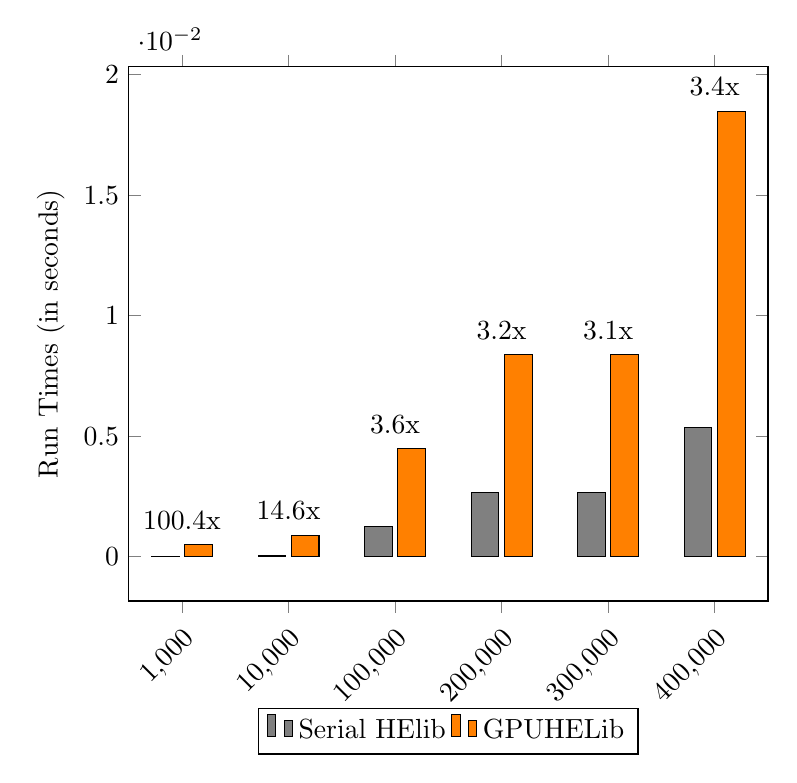
\begin{tikzpicture}

\begin{axis}[
    ybar,
    width=.8\textwidth,
    legend style={at={(0.5,-0.2)},anchor=north,legend columns=-1},
    ylabel=Run Times (in seconds),
    symbolic x coords={$1{,}000$,$10{,}000$,$100{,}000$,$200{,}000$,$300{,}000$,$400{,}000$},
    xtick=data,
    x tick label style={rotate=45,anchor=north east},
]

\addplot[fill=gray]
    coordinates {
    ($1{,}000$,5.000E-06)($10{,}000$,6.150E-05)($100{,}000$,1.259E-03)($200{,}000$,2.644E-03)($300{,}000$,2.674E-03)($400{,}000$,5.366E-03) };
    
\addplot[fill=orange]
    coordinates {
    ($1{,}000$,5.020E-04)($10{,}000$,8.950E-04)($100{,}000$,4.498E-03)($200{,}000$,8.398E-03)($300{,}000$,8.395E-03)($400{,}000$,1.848E-02) };

\node at (axis cs:$1{,}000$,1.50E-03) {100.4x};
\node at (axis cs:$10{,}000$,1.90E-03) {14.6x};
\node at (axis cs:$100{,}000$,5.50E-03) {3.6x};
\node at (axis cs:$200{,}000$,9.40E-03) {3.2x};
\node at (axis cs:$300{,}000$,9.39E-03) {3.1x};
\node at (axis cs:$400{,}000$,1.95E-02) {3.4x};
    
\legend{Serial HElib,GPUHELib}
\end{axis}
\end{tikzpicture}

\caption{Sub Run Times Comparison at Function Level}
\label{fig:level2ComparisonSerialGPUSubVecs}
\end{figure}

\begin{figure}[p]
\centering
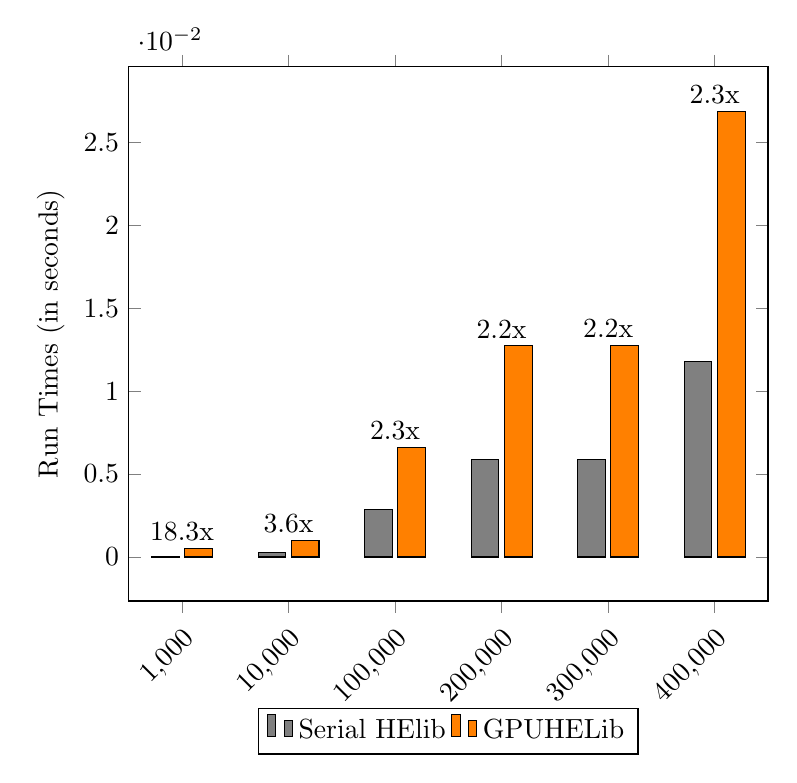
\begin{tikzpicture}

\begin{axis}[
    ybar,
    width=.8\textwidth,
    legend style={at={(0.5,-0.2)},anchor=north,legend columns=-1},
    ylabel=Run Times (in seconds),
    symbolic x coords={$1{,}000$,$10{,}000$,$100{,}000$,$200{,}000$,$300{,}000$,$400{,}000$},
    xtick=data,
    x tick label style={rotate=45,anchor=north east},
]

\addplot[fill=gray]
    coordinates {
    ($1{,}000$,2.900E-05)($10{,}000$,2.830E-04)($100{,}000$,2.879E-03)($200{,}000$,5.863E-03)($300{,}000$,5.856E-03)($400{,}000$,1.176E-02) };
    
\addplot[fill=orange]
    coordinates {
    ($1{,}000$,5.302E-04)($10{,}000$,1.006E-03)($100{,}000$,6.599E-03)($200{,}000$,1.273E-02)($300{,}000$,1.276E-02)($400{,}000$,2.687E-02) };
    					
\node at (axis cs:$1{,}000$,1.53E-03) {18.3x};
\node at (axis cs:$10{,}000$,2.01E-03) {3.6x};
\node at (axis cs:$100{,}000$,7.60E-03) {2.3x};
\node at (axis cs:$200{,}000$,1.37E-02) {2.2x};
\node at (axis cs:$300{,}000$,1.38E-02) {2.2x};
\node at (axis cs:$400{,}000$,2.79E-02) {2.3x};
    
\legend{Serial HElib,GPUHELib}
\end{axis}
\end{tikzpicture}

\caption{Mul Run Times Comparison at Function Level}
\label{fig:level2ComparisonSerialGPUMulVecs}
\end{figure}

Table \ref{tab:GPUserialLevel2Runtimes} and Table \ref{tab:GPULevel2Runtimes} display the run times for the serial HElib and GPUHElib tests respectively. As noted before, both tests were run with input sizes ranging from 1,000 to 400,000.

Figure \ref{fig:level2ComparisonSerialGPUAddVecs}, Figure \ref{fig:level2ComparisonSerialGPUSubVecs}, and Figure \ref{fig:level2ComparisonSerialGPUMulVecs} show the comparisons between the run times for each of the operations at the function level. Also displayed in the figures is the run time slow down of the GPU variant compared to the serial version. For example, in Figure \ref{fig:level2ComparisonSerialGPUAddVecs}, the 104.2x above 1,000 means that the GPU variant took 104.2 times longer to complete compared to the serial version.

All these times again reiterate that for the smaller input sizes, the run times for the GPU variant are vastly larger, almost 100x for addition and subtraction, and about 18x for multiplication. As the input sizes increase, the run times get closer and closer, but minimize at about 3.1x for addition and subtraction and at about 2x for multiplication. Again one can see that for the 400,000 input size, the slow downs increase for all the operations compared to the previous input size, 300,000, going from 3.2x to 3.4x and 3.5x respectively and from 2.2x to 2.3x. The results for the multiplication times make it clear that the speedup seen at the circuit level must be caused by other factors than the GPU implementation of multiplication. These times show that multiplication behaves exactly like the other operations in terms of run time patterns. The cause for these slow downs is evident after examining the recorded times at the phase level.

\subsection{GPUHElib Phase Level Run Times}
\begin{table}[p]
\centering
\begin{tabular}{ | r | r | r | r | r | r | r | }
 \multicolumn{1}{ r }{} & \multicolumn{6}{ c }{$size\_of\_row$} \\ \cline{2-7}
 \multicolumn{1}{ r |}{} & $1{,}000$ & $10{,}000$ & $100{,}000$ & $200{,}000$ & $300{,}000$ & $400{,}000$ \\ \hline
 Setup & 2.420E-04 & 2.465E-04 & 2.848E-04 & 3.013E-04 & 3.015E-04 & 3.133E-04 \\ \hline
 Phase 1 & 9.500E-05 & 2.568E-04 & 2.137E-03 & 4.289E-03 & 4.345E-03 & 1.164E-02 \\ \hline
 Phase 2 & 4.425E-05 & 3.350E-05 & 1.283E-04 & 2.423E-04 & 2.420E-04 & 3.728E-04 \\ \hline
 Phase 3 & 1.373E-04 & 2.900E-04 & 1.837E-03 & 3.420E-03 & 3.454E-03 & 6.308E-03 \\ \hline
\end{tabular}
\caption{GPUHElib Add phase level run times (in seconds)}
\label{tab:GPULevel3RuntimesAddVecs}
\end{table}

\begin{figure}[p]
\centering
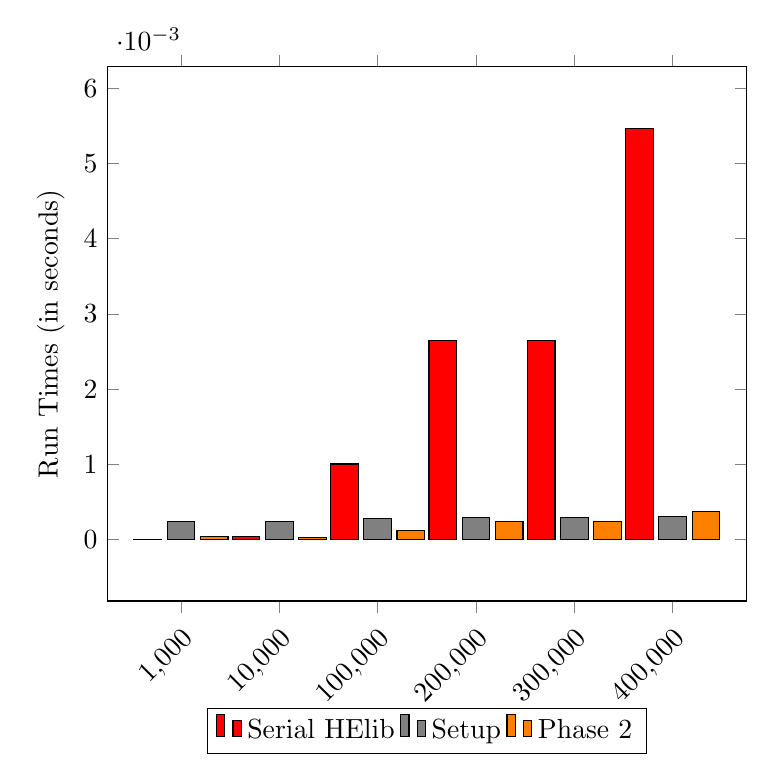
\begin{tikzpicture}

\begin{axis}[
    ybar,
    width=.8\textwidth,
    enlargelimits=0.15,
    legend style={at={(0.5,-0.2)},anchor=north,legend columns=-1},
    ylabel=Run Times (in seconds),
    symbolic x coords={$1{,}000$,$10{,}000$,$100{,}000$,$200{,}000$,$300{,}000$,$400{,}000$},
    xtick=data,
    x tick label style={rotate=45,anchor=north east},
]

\addplot[fill=red]
    coordinates {
    ($1{,}000$,5.000E-06)($10{,}000$,4.825E-05)($100{,}000$,1.007E-03)($200{,}000$,2.648E-03)($300{,}000$,2.653E-03)($400{,}000$,5.466E-03) };
    
\addplot[fill=gray]
    coordinates {
    ($1{,}000$,2.420E-04)($10{,}000$,2.465E-04)($100{,}000$,2.848E-04)($200{,}000$,3.013E-04)($300{,}000$,3.015E-04)($400{,}000$,3.133E-04) };
    
\addplot[fill=orange]
    coordinates {
    ($1{,}000$,4.425E-05)($10{,}000$,3.350E-05)($100{,}000$,1.283E-04)($200{,}000$,2.423E-04)($300{,}000$,2.420E-04)($400{,}000$,3.728E-04) };
    
\legend{Serial HElib,Setup,Phase 2}
\end{axis}
\end{tikzpicture}

\caption{Add Phase Level Run Times Comparison - Operation}
\label{fig:level3ComparisonSerialGPUAddVecs1}
\end{figure}

\begin{figure}[p]
\centering
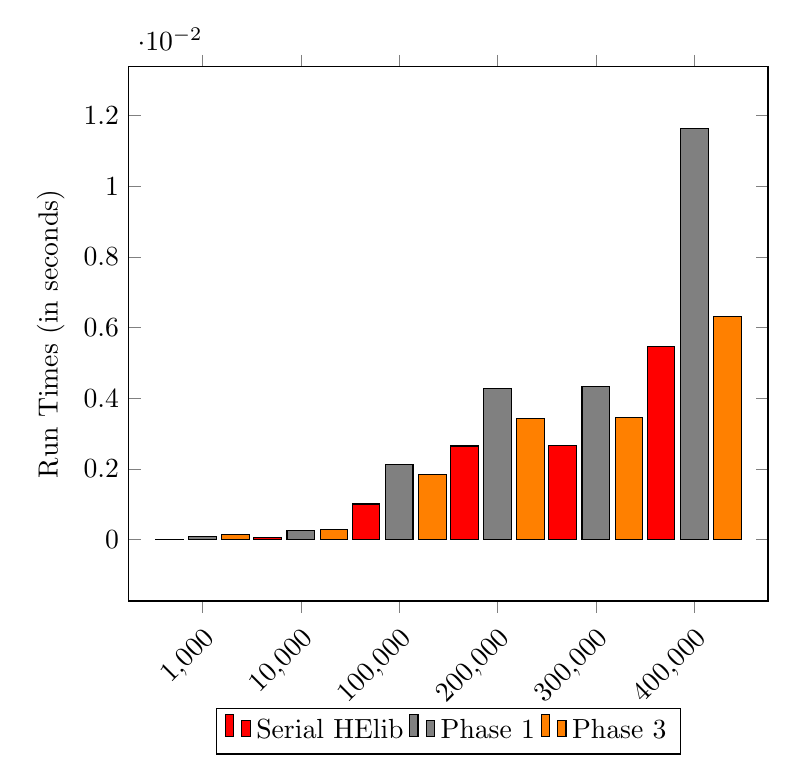
\begin{tikzpicture}

\begin{axis}[
    ybar,
    width=.8\textwidth,
    enlargelimits=0.15,
    legend style={at={(0.5,-0.2)},anchor=north,legend columns=-1},
    ylabel=Run Times (in seconds),
    symbolic x coords={$1{,}000$,$10{,}000$,$100{,}000$,$200{,}000$,$300{,}000$,$400{,}000$},
    xtick=data,
    x tick label style={rotate=45,anchor=north east},
]

\addplot[fill=red]
    coordinates {
    ($1{,}000$,5.000E-06)($10{,}000$,4.825E-05)($100{,}000$,1.007E-03)($200{,}000$,2.648E-03)($300{,}000$,2.653E-03)($400{,}000$,5.466E-03) };
    
\addplot[fill=gray]
    coordinates {
    ($1{,}000$,9.500E-05)($10{,}000$,2.568E-04)($100{,}000$,2.137E-03)($200{,}000$,4.289E-03)($300{,}000$,4.345E-03)($400{,}000$,1.164E-02) };
    
\addplot[fill=orange]
    coordinates {
    ($1{,}000$,1.373E-04)($10{,}000$,2.900E-04)($100{,}000$,1.837E-03)($200{,}000$,3.420E-03)($300{,}000$,3.454E-03)($400{,}000$,6.308E-03) };
    
\legend{Serial HElib,Phase 1,Phase 3}
\end{axis}
\end{tikzpicture}

\caption{Add Phase Level Run Times Comparison - Memory}
\label{fig:level3ComparisonSerialGPUAddVecs2}
\end{figure}

\begin{table}[p]
\centering
\begin{tabular}{ | r | r | r | r | r | r | r | }
 \multicolumn{1}{ r }{} & \multicolumn{6}{ c }{$size\_of\_row$} \\ \cline{2-7}
 \multicolumn{1}{ r |}{} & $1{,}000$ & $10{,}000$ & $100{,}000$ & $200{,}000$ & $300{,}000$ & $400{,}000$ \\ \hline
 Setup & 2.455E-04 & 2.830E-04 & 3.035E-04 & 3.065E-04 & 3.045E-04 & 3.050E-04 \\ \hline
 Phase 1 & 9.000E-05 & 2.535E-04 & 2.262E-03 & 4.377E-03 & 4.377E-03 & 1.152E-02 \\ \hline
 Phase 2 & 3.400E-05 & 4.200E-05 & 1.280E-04 & 2.420E-04 & 2.425E-04 & 3.745E-04 \\ \hline
 Phase 3 & 1.275E-04 & 3.120E-04 & 1.799E-03 & 3.466E-03 & 3.465E-03 & 6.275E-03 \\ \hline
\end{tabular}
\caption{GPUHElib Sub phase level run times (in seconds)}
\label{tab:GPULevel3RuntimesSubVecs}
\end{table}

\begin{figure}[p]
\centering
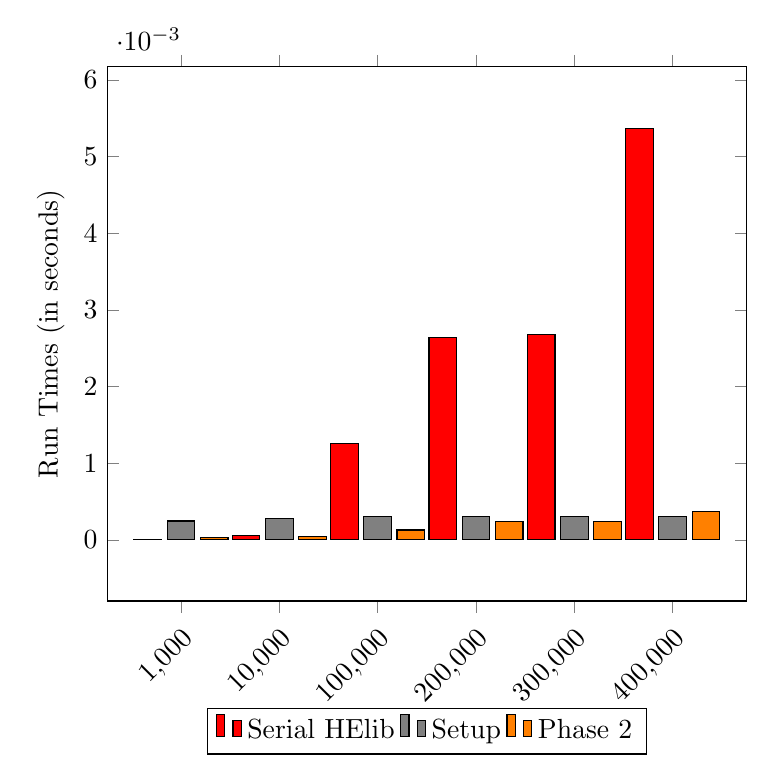
\begin{tikzpicture}

\begin{axis}[
    ybar,
    width=.8\textwidth,
    enlargelimits=0.15,
    legend style={at={(0.5,-0.2)},anchor=north,legend columns=-1},
    ylabel=Run Times (in seconds),
    symbolic x coords={$1{,}000$,$10{,}000$,$100{,}000$,$200{,}000$,$300{,}000$,$400{,}000$},
    xtick=data,
    x tick label style={rotate=45,anchor=north east},
]

\addplot[fill=red]
    coordinates {
    ($1{,}000$,5.000E-06)($10{,}000$,6.150E-05)($100{,}000$,1.259E-03)($200{,}000$,2.644E-03)($300{,}000$,2.674E-03)($400{,}000$,5.366E-03) };
    
\addplot[fill=gray]
    coordinates {
    ($1{,}000$,2.455E-04)($10{,}000$,2.830E-04)($100{,}000$,3.035E-04)($200{,}000$,3.065E-04)($300{,}000$,3.045E-04)($400{,}000$,3.050E-04) };
    
\addplot[fill=orange]
    coordinates {
    ($1{,}000$,3.400E-05)($10{,}000$,4.200E-05)($100{,}000$,1.280E-04)($200{,}000$,2.420E-04)($300{,}000$,2.425E-04)($400{,}000$,3.745E-04) };
    
\legend{Serial HElib,Setup,Phase 2}
\end{axis}
\end{tikzpicture}

\caption{Sub Phase Level Run Times Comparison - Operation}
\label{fig:level3ComparisonSerialGPUSubVecs1}
\end{figure}

\begin{figure}[p]
\centering
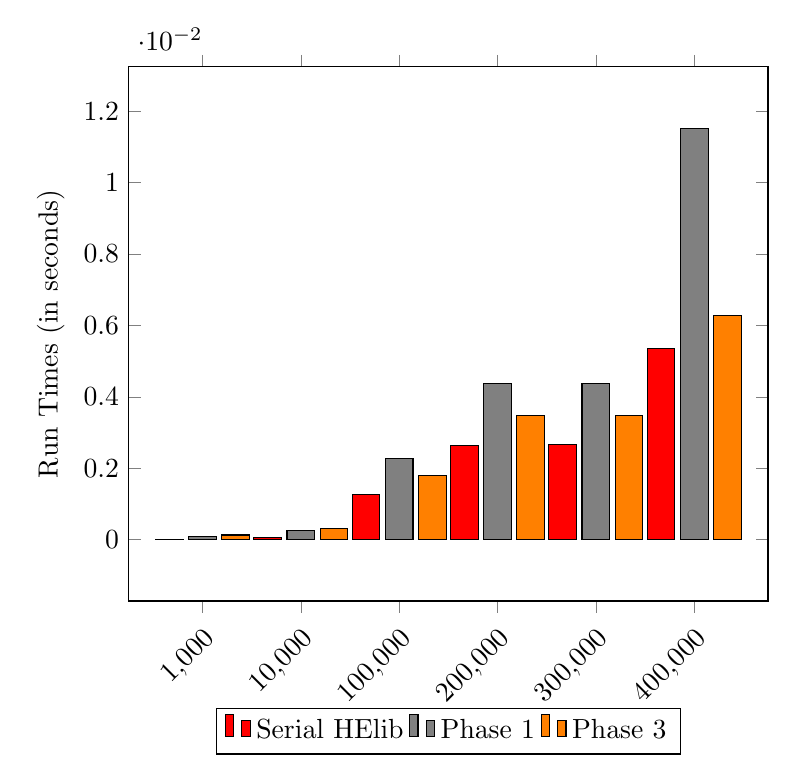
\begin{tikzpicture}

\begin{axis}[
    ybar,
    width=.8\textwidth,
    enlargelimits=0.15,
    legend style={at={(0.5,-0.2)},anchor=north,legend columns=-1},
    ylabel=Run Times (in seconds),
    symbolic x coords={$1{,}000$,$10{,}000$,$100{,}000$,$200{,}000$,$300{,}000$,$400{,}000$},
    xtick=data,
    x tick label style={rotate=45,anchor=north east},
]

\addplot[fill=red]
    coordinates {
    ($1{,}000$,5.000E-06)($10{,}000$,6.150E-05)($100{,}000$,1.259E-03)($200{,}000$,2.644E-03)($300{,}000$,2.674E-03)($400{,}000$,5.366E-03) };
    
\addplot[fill=gray]
    coordinates {
    ($1{,}000$,9.000E-05)($10{,}000$,2.535E-04)($100{,}000$,2.262E-03)($200{,}000$,4.377E-03)($300{,}000$,4.377E-03)($400{,}000$,1.152E-02) };
    
\addplot[fill=orange]
    coordinates {
    ($1{,}000$,1.275E-04)($10{,}000$,3.120E-04)($100{,}000$,1.799E-03)($200{,}000$,3.466E-03)($300{,}000$,3.465E-03)($400{,}000$,6.275E-03) };
    
\legend{Serial HElib,Phase 1,Phase 3}
\end{axis}
\end{tikzpicture}

\caption{Sub Phase Level Run Times Comparison - Memory}
\label{fig:level3ComparisonSerialGPUSubVecs2}
\end{figure}

\begin{table}[p]
\centering
\begin{tabular}{ | r | r | r | r | r | r | r | }
 \multicolumn{1}{ r }{} & \multicolumn{6}{ c }{$size\_of\_row$} \\ \cline{2-7}
 \multicolumn{1}{ r |}{} & $1{,}000$ & $10{,}000$ & $100{,}000$ & $200{,}000$ & $300{,}000$ & $400{,}000$ \\ \hline
 Setup & 2.405E-04 & 2.447E-04 & 3.027E-04 & 3.200E-04 & 3.157E-04 & 3.207E-04 \\ \hline
 Phase 1 & 7.933E-05 & 1.853E-04 & 1.845E-03 & 3.955E-03 & 3.997E-03 & 1.029E-02 \\ \hline
 Phase 2 & 3.000E-05 & 3.183E-05 & 1.247E-04 & 2.398E-04 & 2.353E-04 & 3.508E-04 \\ \hline
 Phase 3 & 1.772E-04 & 5.418E-04 & 4.323E-03 & 8.213E-03 & 8.212E-03 & 1.591E-02 \\ \hline
\end{tabular}
\caption{GPUHElib Mul phase level run times (in seconds)}
\label{tab:GPULevel3RuntimesMulVecs}
\end{table}

\begin{figure}[p]
\centering
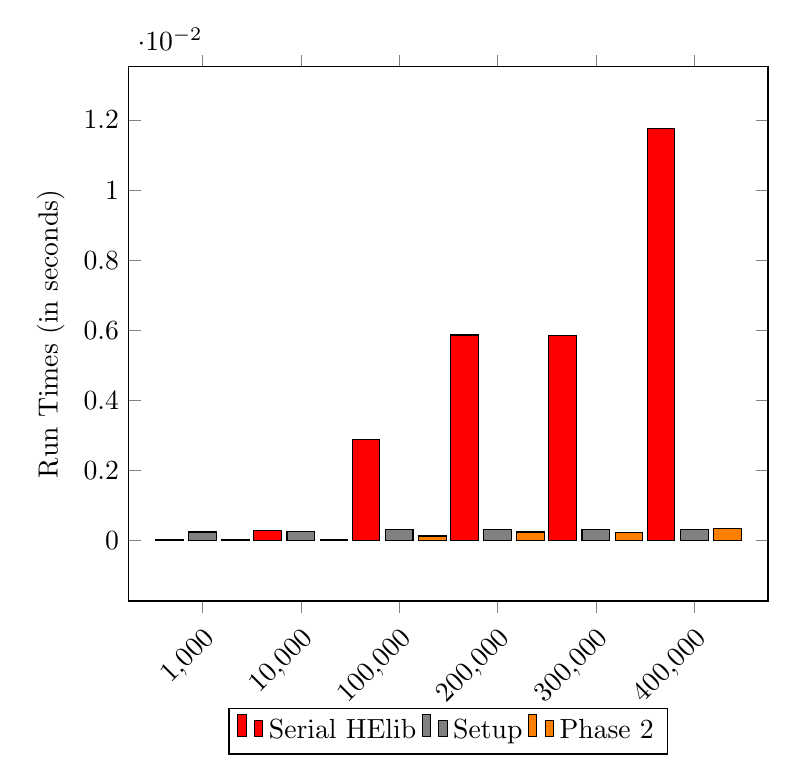
\begin{tikzpicture}

\begin{axis}[
    ybar,
    width=.8\textwidth,
    enlargelimits=0.15,
    legend style={at={(0.5,-0.2)},anchor=north,legend columns=-1},
    ylabel=Run Times (in seconds),
    symbolic x coords={$1{,}000$,$10{,}000$,$100{,}000$,$200{,}000$,$300{,}000$,$400{,}000$},
    xtick=data,
    x tick label style={rotate=45,anchor=north east},
]

\addplot[fill=red]
    coordinates {
    ($1{,}000$,2.900E-05)($10{,}000$,2.830E-04)($100{,}000$,2.879E-03)($200{,}000$,5.863E-03)($300{,}000$,5.856E-03)($400{,}000$,1.176E-02) };
    
\addplot[fill=gray]
    coordinates {
    ($1{,}000$,2.405E-04)($10{,}000$,2.447E-04)($100{,}000$,3.027E-04)($200{,}000$,3.200E-04)($300{,}000$,3.157E-04)($400{,}000$,3.207E-04) };
    
\addplot[fill=orange]
    coordinates {
    ($1{,}000$,3.000E-05)($10{,}000$,3.183E-05)($100{,}000$,1.247E-04)($200{,}000$,2.398E-04)($300{,}000$,2.353E-04)($400{,}000$,3.508E-04) };
    
\legend{Serial HElib,Setup,Phase 2}
\end{axis}
\end{tikzpicture}

\caption{Mul Phase Level Run Times Comparison - Operation}
\label{fig:level3ComparisonSerialGPUMulVecs1}
\end{figure}

\begin{figure}[p]
\centering
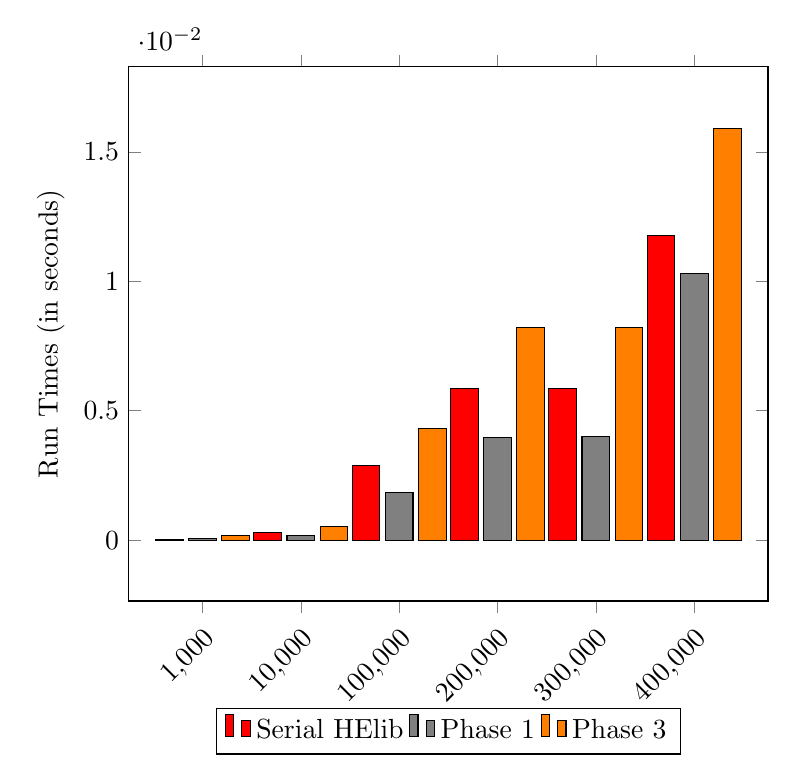
\begin{tikzpicture}

\begin{axis}[
    ybar,
    width=.8\textwidth,
    enlargelimits=0.15,
    legend style={at={(0.5,-0.2)},anchor=north,legend columns=-1},
    ylabel=Run Times (in seconds),
    symbolic x coords={$1{,}000$,$10{,}000$,$100{,}000$,$200{,}000$,$300{,}000$,$400{,}000$},
    xtick=data,
    x tick label style={rotate=45,anchor=north east},
]

\addplot[fill=red]
    coordinates {
    ($1{,}000$,2.900E-05)($10{,}000$,2.830E-04)($100{,}000$,2.879E-03)($200{,}000$,5.863E-03)($300{,}000$,5.856E-03)($400{,}000$,1.176E-02) };
    
\addplot[fill=gray]
    coordinates {
    ($1{,}000$,7.933E-05)($10{,}000$,1.853E-04)($100{,}000$,1.845E-03)($200{,}000$,3.955E-03)($300{,}000$,3.997E-03)($400{,}000$,1.029E-02) };
    
\addplot[fill=orange]
    coordinates {
    ($1{,}000$,1.772E-04)($10{,}000$,5.418E-04)($100{,}000$,4.323E-03)($200{,}000$,8.213E-03)($300{,}000$,8.212E-03)($400{,}000$,1.591E-02) };
    
\legend{Serial HElib,Phase 1,Phase 3}
\end{axis}
\end{tikzpicture}

\caption{Mul Phase Level Run Times Comparison - Memory}
\label{fig:level3ComparisonSerialGPUMulVecs2}
\end{figure}

Table \ref{tab:GPULevel3RuntimesAddVecs}, Table \ref{tab:GPULevel3RuntimesSubVecs}, and Table \ref{tab:GPULevel3RuntimesMulVecs} all display the phase level run times for each operation respectively. The four phases are as follows: setup (vector and stream creation), phase 1 (host to device memory copy), phase 2 (operation on GPU), and phase 3 (device to host memory copy). These times have been split between two plots for each operation. One group of plots focuses on the overall run time of serial HElib compared to the setup and phase 2 times recorded. These are the \say{Operation} plots, Figure \ref{fig:level3ComparisonSerialGPUAddVecs1}, Figure \ref{fig:level3ComparisonSerialGPUSubVecs1}, and Figure \ref{fig:level3ComparisonSerialGPUMulVecs1}. The other group of plots focus on the overhead phases, phase 1 and phase 3, of GPUHElib compared to the overall run time of serial HElib for each operation and are denoted \say{Memory}. These are Figure \ref{fig:level3ComparisonSerialGPUAddVecs2}, Figure \ref{fig:level3ComparisonSerialGPUSubVecs2}, and Figure \ref{fig:level3ComparisonSerialGPUMulVecs2}.

The \say{Operation} plots show the design is working as intended and as all GPU designs are ideally suppose to work. The reliance on the GPU to perform the computation drastically reduces the run time for those phases. Furthermore, as the input size increases largely, the run times for setup and phase 2 only increase slightly. 

The setup phase always took about the same amount of time no matter the input size, only varying by about 8E-05 from the smallest input to the largest. Phase 2 times steadily increased, however not at the rapid pace of the serial HElib versions. This is what is expected when using a GPU to perform operations.

These are the desired results when working with a GPU. The offloading of work onto the GPU allows for the operation portions of the work to drastically decrease in run time. Of course, these results do not characterize the overall recorded times for GPUHElib compared to serial HElib. Therefore something else must be going wrong, causing the run times to be longer than the their serial counterparts.

The \say{Memory} plots show where this design fails. The amount of time needed to move the data back and forth from the GPU is immense. The times for phase 1 and phase 3 are always larger than the entire run time of the serial version for every operation across all input sizes, except for the multiplication operation, where the phase 1 times are actually less than the overall run time of the serial version, but not by much. These times are very disappointing, as they are the reason this design is performing so poorly. Luckily, these times could be lower, given better hardware and possible future work, which could make GPUHElib a viable option. If the problem was in the design or if the run times for the setup or phase 1 were worse, then the total design would not have any hope of being used. But because they are in the memory transfer phases, there is still hope that this design could become viable with further work.

\section{DistrubtedHElib Evaluation Results} \label{sec:DistributedHElibEvaluationResults}
As discussed earlier in this chapter, DistributedHElib has three levels of timing information begin recorded. The highest level is the circuit level in the test program. The next is at the function level, inside \verb|DoubleCRT|. The third and lowest level is the distribute and wait level. This level has two timers which measure the distribute time, the time necessary for the dispatcher node to assign work and partition the data, and the wait time, the time the dispatcher node is waiting for the compute nodes to finish their work and return the results. Additionally three cluster sizes, 4, 8, and 16 nodes, were used during testing The timing results for each of these levels is discussed in more detail below.

\subsection{DistributedHElib Circuit Level Run Times}
\begin{table}[p]
\centering
\begin{tabular}{ | r | r | r | r | r | r | r | }
 \multicolumn{1}{ r }{} & \multicolumn{6}{ c }{$size\_of\_row$} \\ \cline{2-7}
 \multicolumn{1}{ r |}{} & $1{,}000$ & $10{,}000$ & $100{,}000$ & $200{,}000$ & $300{,}000$ & $400{,}000$ \\ \hline
 Add & 1.400E-05 & 1.070E-04 & 2.525E-03 & 5.347E-03 & 5.313E-03 & 1.048E-02 \\ \hline
 Sub & 1.400E-05 & 1.250E-04 & 2.491E-03 & 5.308E-03 & 5.244E-03 & 1.080E-02 \\ \hline
 Mul & 4.996E-03 & 1.030E-01 & 1.151 & 2.644 & 7.286 & 1.202E+01 \\ \hline
\end{tabular}
\caption{Serial HElib circuit level run times (in seconds)}
\label{tab:DistributedserialLevel1Runtimes}
\end{table}

\begin{table}[p]
\centering
\begin{tabular}{ | r | r | r | r | r | r | r | }
 \multicolumn{1}{ r }{} & \multicolumn{6}{ c }{$size\_of\_row$} \\ \cline{2-7}
 \multicolumn{1}{ r |}{} & $1{,}000$ & $10{,}000$ & $100{,}000$ & $200{,}000$ & $300{,}000$ & $400{,}000$ \\ \hline
 Add & 1.457E-03 & 7.496E-03 & 8.933E-02 & 1.783E-01 & 1.550E-01 & 3.455E-01 \\ \hline
 Sub & 1.544E-03 & 7.479E-03 & 7.773E-02 & 1.666E-01 & 1.647E-01 & 3.203E-01 \\ \hline
 Mul & 1.254E-02 & 1.371E-01 & 1.559 & 3.444 & 8.350 & 1.009E+01 \\ \hline
\end{tabular}
\caption{DistributedHElib circuit level run times (in seconds) on 4 nodes}
\label{tab:DistributedLevel1Runtimes4Nodes}
\end{table}

\begin{figure}[p]
\centering

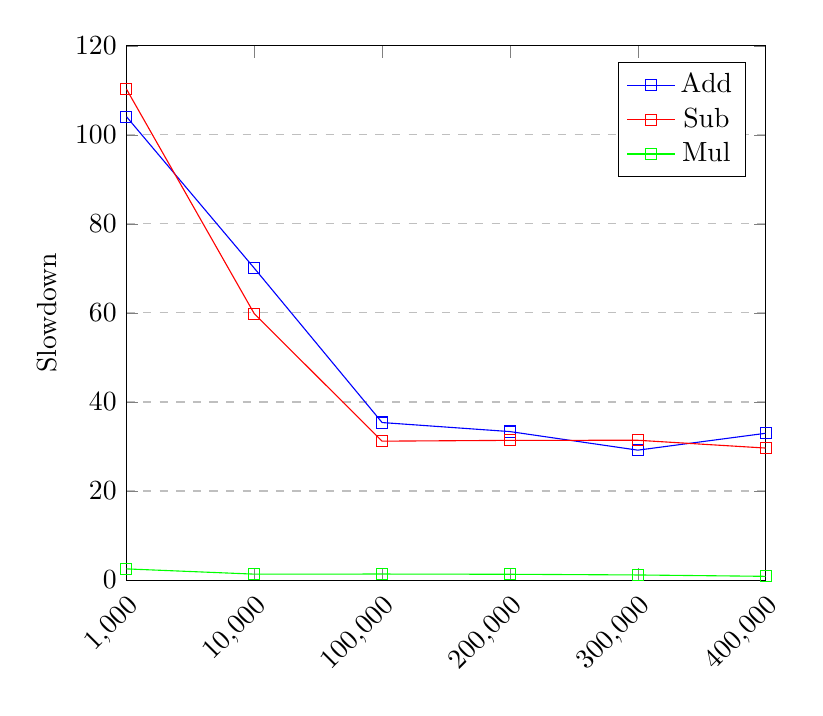
\begin{tikzpicture}
\begin{axis}
[
    ylabel={Slowdown},
    width=.8\textwidth,
    xmin=1, xmax=6,
    ymin=0, ymax=120,
    xtick={1,2,3,4,5,6},
    xticklabels={$1{,}000$, $10{,}000$, $100{,}000$, $200{,}000$, $300{,}000$, $400{,}000$},
    ytick={120,100,80,60,40,20,0},
    legend pos=north east,
    ymajorgrids=true,
    grid style=dashed,
    x tick label style={rotate=45,anchor=north east},
]

\addplot[color=blue,mark=square]
    coordinates {
    (1,1.041E+02)(2,7.006E+01)(3,3.538E+01)(4,3.335E+01)(5,2.918E+01)(6,3.297E+01) };
    
\addplot[color=red,mark=square]
    coordinates {
    (1,1.103E+02)(2,5.983E+01)(3,3.120E+01)(4,3.138E+01)(5,3.140E+01)(6,2.965E+01) };

\addplot[color=green,mark=square]
    coordinates {
    (1,2.510E+00)(2,1.332E+00)(3,1.354E+00)(4,1.302E+00)(5,1.146E+00)(6,8.393E-01) };
    
\legend{Add,Sub,Mul}
 
\end{axis}
\end{tikzpicture}

\caption{Run Time Comparison at Circuit Level on 4 Nodes}
\label{fig:level1ComparisonSerialDistributed4Nodes}
\end{figure}

\begin{table}[p]
\centering
\begin{tabular}{ | r | r | r | r | r | r | r | }
 \multicolumn{1}{ r }{} & \multicolumn{6}{ c }{$size\_of\_row$} \\ \cline{2-7}
 \multicolumn{1}{ r |}{} & $1{,}000$ & $10{,}000$ & $100{,}000$ & $200{,}000$ & $300{,}000$ & $400{,}000$ \\ \hline
 Add & 1.712E-03 & 9.161E-03 & 1.076E-01 & 2.228E-01 & 2.266E-01 & 4.540E-01 \\ \hline
 Sub & 1.791E-03 & 9.219E-03 & 1.117E-01 & 2.113E-01 & 2.139E-01 & 4.560E-01 \\ \hline
 Mul & 1.350E-02 & 1.454E-01 & 1.666 & 3.689 & 8.589 & 1.136E+01 \\ \hline
\end{tabular}
\caption{DistributedHElib circuit level run times (in seconds) on 8 nodes}
\label{tab:DistributedLevel1Runtimes8Nodes}
\end{table}

\begin{figure}[p]
\centering

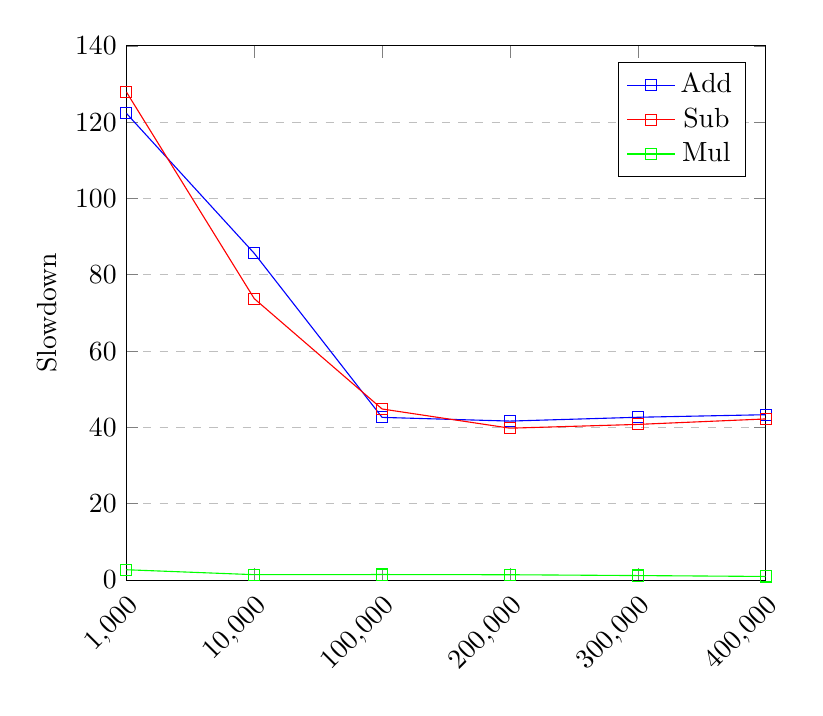
\begin{tikzpicture}
\begin{axis}
[
    ylabel={Slowdown},
    width=.8\textwidth,
    xmin=1, xmax=6,
    ymin=0, ymax=140,
    xtick={1,2,3,4,5,6},
    xticklabels={$1{,}000$, $10{,}000$, $100{,}000$, $200{,}000$, $300{,}000$, $400{,}000$},
    ytick={140,120,100,80,60,40,20,0},
    legend pos=north east,
    ymajorgrids=true,
    grid style=dashed,
    x tick label style={rotate=45,anchor=north east},
]

\addplot[color=blue,mark=square]
    coordinates {
    (1,1.223E+02)(2,8.562E+01)(3,4.263E+01)(4,4.166E+01)(5,4.266E+01)(6,4.333E+01) };
    
\addplot[color=red,mark=square]
    coordinates {
    (1,1.279E+02)(2,7.375E+01)(3,4.483E+01)(4,3.980E+01)(5,4.079E+01)(6,4.222E+01) };

\addplot[color=green,mark=square]
    coordinates {
    (1,2.703E+00)(2,1.412E+00)(3,1.447E+00)(4,1.395E+00)(5,1.179E+00)(6,9.451E-01) };
    
\legend{Add,Sub,Mul}
 
\end{axis}
\end{tikzpicture}

\caption{Run Time Comparison at Circuit Level on 8 Nodes}
\label{fig:level1ComparisonSerialDistributed8Nodes}
\end{figure}

\begin{table}[p]
\centering
\begin{tabular}{ | r | r | r | r | r | r | r | }
 \multicolumn{1}{ r }{} & \multicolumn{6}{ c }{$size\_of\_row$} \\ \cline{2-7}
 \multicolumn{1}{ r |}{} & $1{,}000$ & $10{,}000$ & $100{,}000$ & $200{,}000$ & $300{,}000$ & $400{,}000$ \\ \hline
 Add & 1.772E-03 & 9.960E-03 & 1.187E-01 & 2.391E-01 & 2.390E-01 & 4.911E-01 \\ \hline
 Sub & 1.850E-03 & 9.741E-03 & 1.194E-01 & 2.398E-01 & 2.364E-01 & 4.744E-01 \\ \hline
 Mul & 2.484E-02 & 1.623E-01 & 1.717 & 3.811 & 8.664 & 1.135E+01 \\ \hline
\end{tabular}
\caption{DistributedHElib circuit level run times (in seconds) on 16 nodes}
\label{tab:DistributedLevel1Runtimes16Nodes}
\end{table}

\begin{figure}[p]
\centering

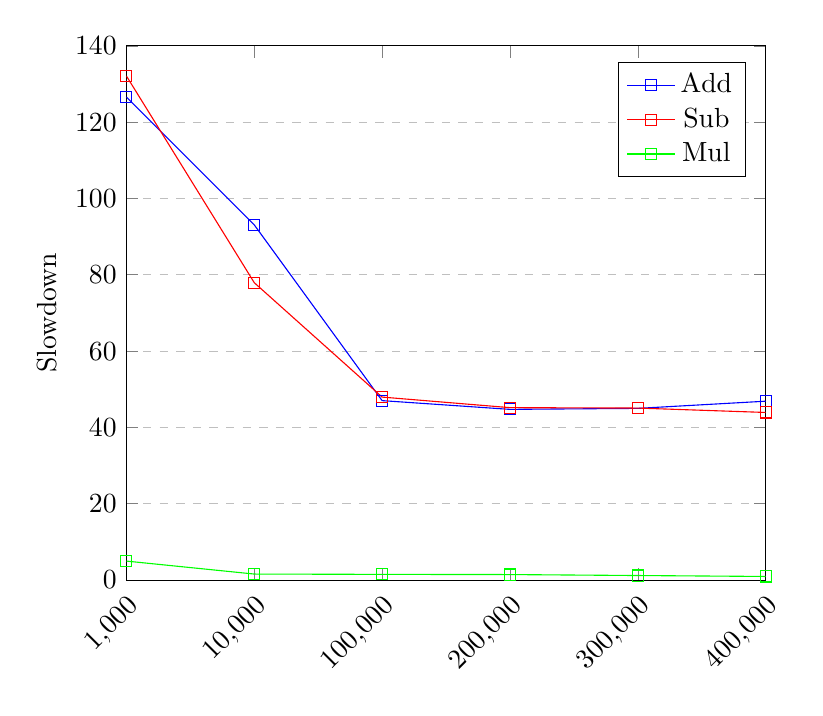
\begin{tikzpicture}
\begin{axis}
[
    ylabel={Slowdown},
    width=.8\textwidth,
    xmin=1, xmax=6,
    ymin=0, ymax=140,
    xtick={1,2,3,4,5,6},
    xticklabels={$1{,}000$, $10{,}000$, $100{,}000$, $200{,}000$, $300{,}000$, $400{,}000$},
    ytick={140,120,100,80,60,40,20,0},
    legend pos=north east,
    ymajorgrids=true,
    grid style=dashed,
    x tick label style={rotate=45,anchor=north east},
]

\addplot[color=blue,mark=square]
    coordinates {
    (1,1.266E+02)(2,9.308E+01)(3,4.702E+01)(4,4.473E+01)(5,4.499E+01)(6,4.687E+01) };
    
\addplot[color=red,mark=square]
    coordinates {
    (1,1.321E+02)(2,7.793E+01)(3,4.795E+01)(4,4.518E+01)(5,4.507E+01)(6,4.392E+01) };

\addplot[color=green,mark=square]
    coordinates {
    (1,4.971E+00)(2,1.576E+00)(3,1.491E+00)(4,1.441E+00)(5,1.189E+00)(6,9.438E-01) };
    
\legend{Add,Sub,Mul}
 
\end{axis}
\end{tikzpicture}

\caption{Run Time Comparison at Circuit Level on 16 Nodes}
\label{fig:level1ComparisonSerialDistributed16Nodes}
\end{figure}

Table \ref{tab:DistributedserialLevel1Runtimes}, Table \ref{tab:DistributedLevel1Runtimes4Nodes}, Table \ref{tab:DistributedLevel1Runtimes8Nodes}, and Table \ref{tab:DistributedLevel1Runtimes16Nodes} display the run times for serial HElib and DistributedHElib tests. Both tests were run with inputs sizes starting at 1,000 and increasing until 400,000. The clusters sizes were 4, 8, and 16 nodes.

Figure \ref{fig:level1ComparisonSerialDistributed4Nodes}, Figure \ref{fig:level1ComparisonSerialDistributed8Nodes}, and Figure \ref{fig:level1ComparisonSerialDistributed16Nodes} visualize these times as the slowdown of DistributedHElib over serial HElib. A value of 1 means that the serial version and the distributed version had the same run time. Above 1 means that the distributed design has a slower run time, and below 1 means that the distributed version has a faster run time.

One can see in these figures that for the smaller input sizes, the run times for addition and subtraction across all cluster sizes are much larger for the distributed design compared to the serial design. These operations take over 100 times as long to complete as their serial counterparts. The multiplication operation also takes longer, however only about 2.5 to 5 times as long depending on the number of nodes in the cluster. 

As the input sizes increase, the addition and subtraction operation slowdowns decrease, until they plateau at around 35, 40, and 45 times as long for the 4, 8, and 16 node clusters respectively. Once they reach these slowdowns, they bounce around, but never continue on the downward trajectory they had for the first few input size increases. The multiplication operation on the other hand always decreases as the input size increases. As the input sizes increase, the multiplication slowdowns approach 1, and at the 400,000 size input, all three cluster sizes dive below 1. The cluster size of 4 has the best results, having about a .84 slowdown, with the other two sizes, 8 and 16, having about a .94. These results mean, for the 400,000 input size, the distributed variant of HElib had faster run times than the serial version across all cluster sizes. Similar to the GPU results, while these times look good, further examination of the lower level tests show that this speed up is probably not happening because of the distributed design, but because of other factors. Next the function level times are examined.

\subsection{DistributedHElib Function Level Run Times}
\begin{table}[p]
\centering
\begin{tabular}{ | r | r | r | r | r | r | r | }
 \multicolumn{1}{ r }{} & \multicolumn{6}{ c }{$size\_of\_row$} \\ \cline{2-7}
 \multicolumn{1}{ r |}{} & $1{,}000$ & $10{,}000$ & $100{,}000$ & $200{,}000$ & $300{,}000$ & $400{,}000$ \\ \hline
 Add & 5.000E-06 & 4.800E-05 & 9.873E-04 & 2.588E-03 & 2.611E-03 & 5.457E-03 \\ \hline
 Sub & 5.000E-06 & 5.850E-05 & 1.238E-03 & 2.646E-03 & 2.614E-03 & 5.391E-03 \\ \hline
 Mul & 2.967E-05 & 2.838E-04 & 2.887E-03 & 5.845E-03 & 5.850E-03 & 1.183E-02 \\ \hline
\end{tabular}
\caption{Serial HElib function level run times (in seconds)}
\label{tab:DistributedserialLevel2Runtimes}
\end{table}

\begin{table}[p]
\centering
\begin{tabular}{ | r | r | r | r | r | r | r | }
 \multicolumn{1}{ r }{} & \multicolumn{6}{ c }{$size\_of\_row$} \\ \cline{2-7}
 \multicolumn{1}{ r |}{} & $1{,}000$ & $10{,}000$ & $100{,}000$ & $200{,}000$ & $300{,}000$ & $400{,}000$ \\ \hline
 Add & 7.423E-04 & 3.604E-03 & 4.898E-02 & 8.503E-02 & 8.048E-02 & 1.764E-01 \\ \hline
 Sub & 7.695E-04 & 3.735E-03 & 3.886E-02 & 8.329E-02 & 8.233E-02 & 1.601E-01 \\ \hline
 Mul & 7.148E-04 & 3.298E-03 & 3.517E-02 & 7.759E-02 & 7.771E-02 & 1.482E-01 \\ \hline
\end{tabular}
\caption{DistributedHElib function level run times (in seconds) on 4 nodes}
\label{tab:DistributedLevel2Runtimes4Nodes}
\end{table}

\begin{table}[p]
\centering
\begin{tabular}{ | r | r | r | r | r | r | r | }
 \multicolumn{1}{ r }{} & \multicolumn{6}{ c }{$size\_of\_row$} \\ \cline{2-7}
 \multicolumn{1}{ r |}{} & $1{,}000$ & $10{,}000$ & $100{,}000$ & $200{,}000$ & $300{,}000$ & $400{,}000$ \\ \hline
 Add & 8.698E-04 & 4.427E-03 & 5.489E-02 & 1.124E-01 & 1.125E-01 & 2.186E-01 \\ \hline
 Sub & 8.930E-04 & 4.427E-03 & 5.583E-02 & 1.056E-01 & 1.069E-01 & 2.280E-01 \\ \hline
 Mul & 8.055E-04 & 4.032E-03 & 4.830E-02 & 9.798E-02 & 9.804E-02 & 1.951E-01 \\ \hline
\end{tabular}
\caption{DistributedHElib function level run times (in seconds) on 8 nodes}
\label{tab:DistributedLevel2Runtimes8Nodes}
\end{table}

\begin{table}[p]
\centering
\begin{tabular}{ | r | r | r | r | r | r | r | }
 \multicolumn{1}{ r }{} & \multicolumn{6}{ c }{$size\_of\_row$} \\ \cline{2-7}
 \multicolumn{1}{ r |}{} & $1{,}000$ & $10{,}000$ & $100{,}000$ & $200{,}000$ & $300{,}000$ & $400{,}000$ \\ \hline
 Add & 9.180E-04 & 7.439E-03 & 5.794E-02 & 1.166E-01 & 1.152E-01 & 2.316E-01 \\ \hline
 Sub & 9.220E-04 & 4.866E-03 & 5.971E-02 & 1.199E-01 & 1.182E-01 & 2.372E-01 \\ \hline
 Mul & 8.373E-04 & 4.498E-03 & 5.036E-02 & 1.025E-01 & 1.054E-01 & 2.126E-01 \\ \hline
\end{tabular}
\caption{DistributedHElib function level run times (in seconds) on 16 nodes}
\label{tab:DistributedLevel2Runtimes16Nodes}
\end{table}

\begin{figure}[p]
\centering
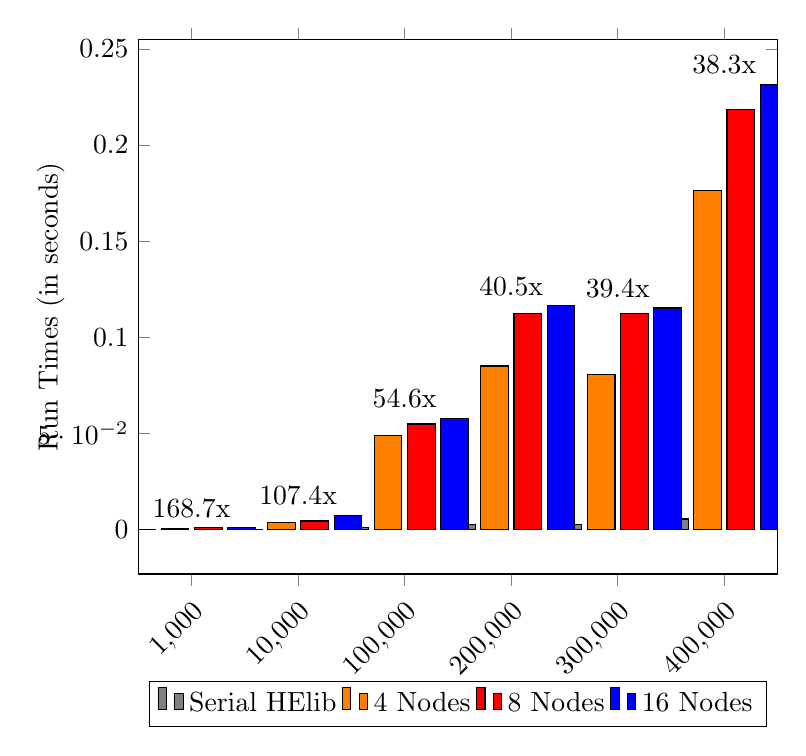
\begin{tikzpicture}

\begin{axis}[
    ybar,
    width=.8\textwidth,
    legend style={at={(0.5,-0.2)},anchor=north,legend columns=-1},
    ylabel=Run Times (in seconds),
    symbolic x coords={$1{,}000$,$10{,}000$,$100{,}000$,$200{,}000$,$300{,}000$,$400{,}000$},
    xtick=data,
    x tick label style={rotate=45,anchor=north east},
    y label style={at={(axis description cs:-0.1,0.5)}, anchor=south},
]

\addplot[fill=gray]
    coordinates {
    ($1{,}000$,5.000E-06)($10{,}000$,4.800E-05)($100{,}000$,9.873E-04)($200{,}000$,2.588E-03)($300{,}000$,2.611E-03)($400{,}000$,5.457E-03) };
    
\addplot[fill=orange]
    coordinates {
    ($1{,}000$,7.423E-04)($10{,}000$,3.604E-03)($100{,}000$,4.898E-02)($200{,}000$,8.503E-02)($300{,}000$,8.048E-02)($400{,}000$,1.764E-01) };
    
\addplot[fill=red]
    coordinates {
    ($1{,}000$,8.698E-04)($10{,}000$,4.427E-03)($100{,}000$,5.489E-02)($200{,}000$,1.124E-01)($300{,}000$,1.125E-01)($400{,}000$,2.186E-01) };
    
\addplot[fill=blue]
    coordinates {
    ($1{,}000$,9.180E-04)($10{,}000$,7.439E-03)($100{,}000$,5.794E-02)($200{,}000$,1.166E-01)($300{,}000$,1.152E-01)($400{,}000$,2.316E-01) };

\node at (axis cs:$1{,}000$,1.092E-02) {168.7x};
\node at (axis cs:$10{,}000$,1.744E-02) {107.4x};
\node at (axis cs:$100{,}000$,6.794E-02) {54.6x};
\node at (axis cs:$200{,}000$,1.266E-01) {40.5x};
\node at (axis cs:$300{,}000$,1.252E-01) {39.4x};
\node at (axis cs:$400{,}000$,2.416E-01) {38.3x};
    
\legend{Serial HElib,4 Nodes,8 Nodes,16 Nodes}
\end{axis}
\end{tikzpicture}

\caption{Add Run Times Comparison at Function Level}
\label{fig:level2ComparisonSerialDistributedAddVecs}
\end{figure}

\begin{figure}[p]
\centering
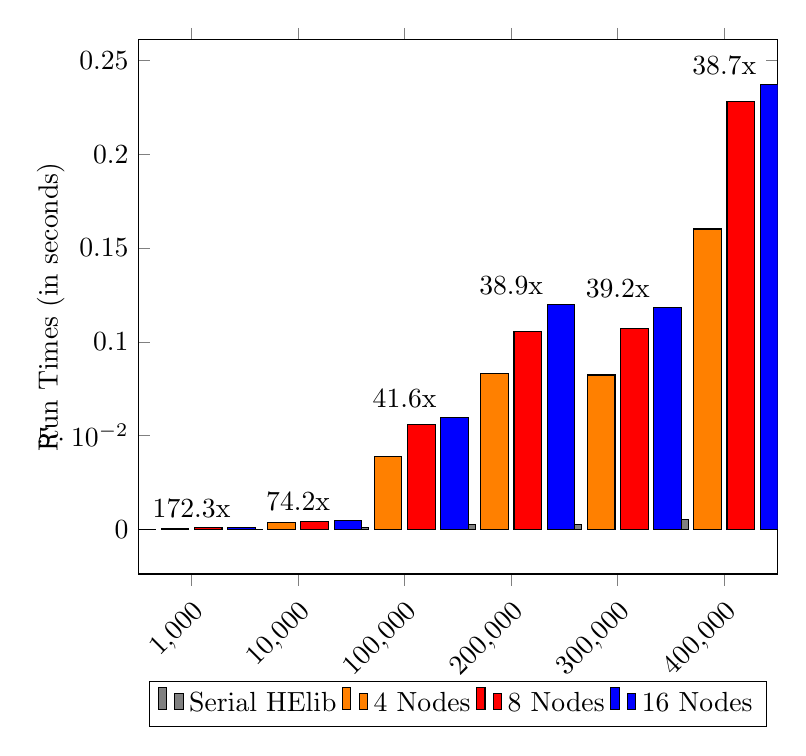
\begin{tikzpicture}

\begin{axis}[
    ybar,
    width=.8\textwidth,
    legend style={at={(0.5,-0.2)},anchor=north,legend columns=-1},
    ylabel=Run Times (in seconds),
    symbolic x coords={$1{,}000$,$10{,}000$,$100{,}000$,$200{,}000$,$300{,}000$,$400{,}000$},
    xtick=data,
    x tick label style={rotate=45,anchor=north east},
    y label style={at={(axis description cs:-0.1,0.5)}, anchor=south},
]

\addplot[fill=gray]
    coordinates {
    ($1{,}000$,5.000E-06)($10{,}000$,5.850E-05)($100{,}000$,1.238E-03)($200{,}000$,2.646E-03)($300{,}000$,2.614E-03)($400{,}000$,5.391E-03) };
    
\addplot[fill=orange]
    coordinates {
    ($1{,}000$,7.695E-04)($10{,}000$,3.735E-03)($100{,}000$,3.886E-02)($200{,}000$,8.329E-02)($300{,}000$,8.233E-02)($400{,}000$,1.601E-01) };
    
\addplot[fill=red]
    coordinates {
    ($1{,}000$,8.930E-04)($10{,}000$,4.427E-03)($100{,}000$,5.583E-02)($200{,}000$,1.056E-01)($300{,}000$,1.069E-01)($400{,}000$,2.280E-01) };
    
\addplot[fill=blue]
    coordinates {
    ($1{,}000$,9.220E-04)($10{,}000$,4.866E-03)($100{,}000$,5.971E-02)($200{,}000$,1.199E-01)($300{,}000$,1.182E-01)($400{,}000$,2.372E-01) };
    
\node at (axis cs:$1{,}000$,1.092E-02) {172.3x};
\node at (axis cs:$10{,}000$,1.487E-02) {74.2x};
\node at (axis cs:$100{,}000$,6.971E-02) {41.6x};
\node at (axis cs:$200{,}000$,1.299E-01) {38.9x};
\node at (axis cs:$300{,}000$,1.282E-01) {39.2x};
\node at (axis cs:$400{,}000$,2.472E-01) {38.7x};
    
\legend{Serial HElib,4 Nodes,8 Nodes,16 Nodes}
\end{axis}
\end{tikzpicture}

\caption{Sub Run Times Comparison at Function Level}
\label{fig:level2ComparisonSerialDistributedSubVecs}
\end{figure}

\begin{figure}[p]
\centering
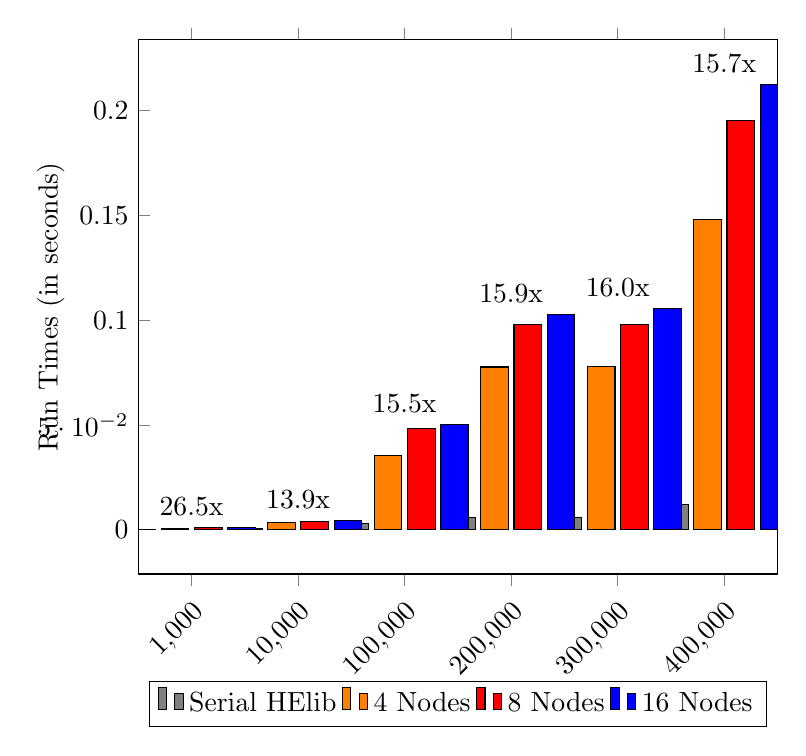
\begin{tikzpicture}

\begin{axis}[
    ybar,
    width=.8\textwidth,
    legend style={at={(0.5,-0.2)},anchor=north,legend columns=-1},
    ylabel=Run Times (in seconds),
    symbolic x coords={$1{,}000$,$10{,}000$,$100{,}000$,$200{,}000$,$300{,}000$,$400{,}000$},
    xtick=data,
    x tick label style={rotate=45,anchor=north east},
    y label style={at={(axis description cs:-0.1,0.5)}, anchor=south},
]

\addplot[fill=gray]
    coordinates {
    ($1{,}000$,2.967E-05)($10{,}000$,2.838E-04)($100{,}000$,2.887E-03)($200{,}000$,5.845E-03)($300{,}000$,5.850E-03)($400{,}000$,1.183E-02) };
    
\addplot[fill=orange]
    coordinates {
    ($1{,}000$,7.148E-04)($10{,}000$,3.298E-03)($100{,}000$,3.517E-02)($200{,}000$,7.759E-02)($300{,}000$,7.771E-02)($400{,}000$,1.482E-01) };
    
\addplot[fill=red]
    coordinates {
    ($1{,}000$,8.055E-04)($10{,}000$,4.032E-03)($100{,}000$,4.830E-02)($200{,}000$,9.798E-02)($300{,}000$,9.804E-02)($400{,}000$,1.951E-01) };
    
\addplot[fill=blue]
    coordinates {
    					
    ($1{,}000$,8.373E-04)($10{,}000$,4.498E-03)($100{,}000$,5.036E-02)($200{,}000$,1.025E-01)($300{,}000$,1.054E-01)($400{,}000$,2.126E-01) };
    
    2.649E+01	1.389E+01	1.545E+01	1.586E+01	1.602E+01	1.566E+01
\node at (axis cs:$1{,}000$,1.084E-02) {26.5x};
\node at (axis cs:$10{,}000$,1.450E-02) {13.9x};
\node at (axis cs:$100{,}000$,6.036E-02) {15.5x};
\node at (axis cs:$200{,}000$,1.125E-01) {15.9x};
\node at (axis cs:$300{,}000$,1.154E-01) {16.0x};
\node at (axis cs:$400{,}000$,2.226E-01) {15.7x};
    
\legend{Serial HElib,4 Nodes,8 Nodes,16 Nodes}
\end{axis}
\end{tikzpicture}

\caption{Mul Run Times Comparison at Function Level}
\label{fig:level2ComparisonSerialDistributedMulVecs}
\end{figure}

Table \ref{tab:DistributedserialLevel2Runtimes}, Table \ref{tab:DistributedLevel2Runtimes4Nodes}, Table \ref{tab:DistributedLevel2Runtimes8Nodes}, and Table \ref{tab:DistributedLevel2Runtimes16Nodes} display the run times at the function level for serial HElib and DistributedHElib on 4, 8, and 16 nodes. 

Figure \ref{fig:level2ComparisonSerialDistributedAddVecs}, Figure \ref{fig:level2ComparisonSerialDistributedSubVecs}, and Figure \ref{fig:level2ComparisonSerialDistributedMulVecs} show the comparisons between the run times for each of the operations at the function level across all variants and cluster sizes. Also displayed in the figures is the average run time slow down, across all cluster sizes, of the distributed variant compared to the serial version. So, for example, in Figure \ref{fig:level2ComparisonSerialDistributedAddVecs}, the 168.7x above 1,000 means that the distributed variant took 168.7 times longer to complete compared to the serial version.

Again for the smaller inputs, these figures show that the distributed variant takes much longer to complete compared to the serial version. For addition and subtraction, the operations take about 170 times as long, and for multiplication, about 25 times as long. As the input sizes increase, the slow downs do decline, however level out around the 200,000 size input. The addition and subtraction operations level out at about 40x, and the multiplication operation levels out at about 16x. Again one can see that the run times plateau for the addition and subtraction operations, just as they did at the circuit level. The results for the multiplication operation at this level show it also has this characteristic, whereas at the circuit level, this characteristic was not observed. Thus the results observed at the circuit level must not be the result of the distributed design, but something else. By looking at the distribute and wait times at level 3, one can understand why these results are occurring.

\subsection{DistributedHElib Distribute and Wait Run Times}
\begin{table}[p]
\centering
\begin{tabular}{ | r | r | r | r | r | r | r | }
 \multicolumn{1}{ r }{} & \multicolumn{6}{ c }{$size\_of\_row$} \\ \cline{2-7}
 \multicolumn{1}{ r |}{} & $1{,}000$ & $10{,}000$ & $100{,}000$ & $200{,}000$ & $300{,}000$ & $400{,}000$ \\ \hline
 Add & 2.240E-04 & 4.638E-04 & 2.373E-04 & 2.500E-04 & 2.438E-04 & 2.698E-04 \\ \hline
 Sub & 2.405E-04 & 5.700E-04 & 2.470E-04 & 2.760E-04 & 2.995E-04 & 2.340E-04 \\ \hline
 Mul & 2.015E-04 & 4.190E-04 & 2.150E-04 & 2.585E-04 & 2.668E-04 & 2.700E-04 \\ \hline
\end{tabular}
\caption{DistributedHElib distribute run times (in seconds) on 4 nodes}
\label{tab:DistributedLevel3RuntimesDistribute4Nodes}
\end{table}

\begin{table}[p]
\centering
\begin{tabular}{ | r | r | r | r | r | r | r | }
 \multicolumn{1}{ r }{} & \multicolumn{6}{ c }{$size\_of\_row$} \\ \cline{2-7}
 \multicolumn{1}{ r |}{} & $1{,}000$ & $10{,}000$ & $100{,}000$ & $200{,}000$ & $300{,}000$ & $400{,}000$ \\ \hline
 Add & 5.158E-04 & 3.137E-03 & 4.874E-02 & 8.478E-02 & 8.023E-02 & 1.761E-01 \\ \hline
 Sub & 5.260E-04 & 3.162E-03 & 3.861E-02 & 8.301E-02 & 8.203E-02 & 1.599E-01 \\ \hline
 Mul & 5.110E-04 & 2.875E-03 & 3.495E-02 & 7.733E-02 & 7.744E-02 & 1.479E-01 \\ \hline
\end{tabular}
\caption{DistributedHElib sync run times (in seconds) on 4 nodes}
\label{tab:DistributedLevel3RuntimesSync4Nodes}
\end{table}

\begin{table}[p]
\centering
\begin{tabular}{ | r | r | r | r | r | r | r | }
 \multicolumn{1}{ r }{} & \multicolumn{6}{ c }{$size\_of\_row$} \\ \cline{2-7}
 \multicolumn{1}{ r |}{} & $1{,}000$ & $10{,}000$ & $100{,}000$ & $200{,}000$ & $300{,}000$ & $400{,}000$ \\ \hline
 Add & 2.773E-04 & 6.288E-04 & 2.740E-04 & 2.978E-04 & 2.913E-04 & 3.055E-04 \\ \hline
 Sub & 2.915E-04 & 7.465E-04 & 3.015E-04 & 2.950E-04 & 2.955E-04 & 3.085E-04 \\ \hline
 Mul & 2.427E-04 & 5.405E-04 & 2.872E-04 & 3.077E-04 & 2.953E-04 & 3.198E-04 \\ \hline
\end{tabular}
\caption{DistributedHElib distribute run times (in seconds) on 8 nodes}
\label{tab:DistributedLevel3RuntimesDistribute8Nodes}
\end{table}

\begin{table}[p]
\centering
\begin{tabular}{ | r | r | r | r | r | r | r | }
 \multicolumn{1}{ r }{} & \multicolumn{6}{ c }{$size\_of\_row$} \\ \cline{2-7}
 \multicolumn{1}{ r |}{} & $1{,}000$ & $10{,}000$ & $100{,}000$ & $200{,}000$ & $300{,}000$ & $400{,}000$ \\ \hline
 Add & 5.903E-04 & 3.796E-03 & 5.461E-02 & 1.121E-01 & 1.122E-01 & 2.183E-01 \\ \hline
 Sub & 5.940E-04 & 3.855E-03 & 5.553E-02 & 1.053E-01 & 1.066E-01 & 2.277E-01 \\ \hline
 Mul & 5.608E-04 & 3.490E-03 & 4.801E-02 & 9.767E-02 & 9.774E-02 & 1.948E-01 \\ \hline
\end{tabular}
\caption{DistributedHElib sync run times (in seconds) on 8 nodes}
\label{tab:DistributedLevel3RuntimesSync8Nodes}
\end{table}

\begin{table}[p]
\centering
\begin{tabular}{ | r | r | r | r | r | r | r | }
 \multicolumn{1}{ r }{} & \multicolumn{6}{ c }{$size\_of\_row$} \\ \cline{2-7}
 \multicolumn{1}{ r |}{} & $1{,}000$ & $10{,}000$ & $100{,}000$ & $200{,}000$ & $300{,}000$ & $400{,}000$ \\ \hline
 Add & 2.985E-04 & 7.418E-04 & 2.923E-04 & 3.083E-04 & 3.515E-04 & 3.235E-04 \\ \hline
 Sub & 3.130E-04 & 8.175E-04 & 3.270E-04 & 3.190E-04 & 3.270E-04 & 3.445E-04 \\ \hline
 Mul & 2.548E-04 & 6.265E-04 & 2.853E-04 & 3.130E-04 & 3.157E-04 & 3.338E-04 \\ \hline
\end{tabular}
\caption{DistributedHElib distribute run times (in seconds) on 16 nodes}
\label{tab:DistributedLevel3RuntimesDistribute16Nodes}
\end{table}

\begin{table}[p]
\centering
\begin{tabular}{ | r | r | r | r | r | r | r | }
 \multicolumn{1}{ r }{} & \multicolumn{6}{ c }{$size\_of\_row$} \\ \cline{2-7}
 \multicolumn{1}{ r |}{} & $1{,}000$ & $10{,}000$ & $100{,}000$ & $200{,}000$ & $300{,}000$ & $400{,}000$ \\ \hline
 Add & 6.178E-04 & 6.692E-03 & 5.765E-02 & 1.163E-01 & 1.149E-01 & 2.313E-01 \\ \hline
 Sub & 6.060E-04 & 4.045E-03 & 5.938E-02 & 1.196E-01 & 1.178E-01 & 2.368E-01 \\ \hline
 Mul & 5.807E-04 & 3.869E-03 & 5.007E-02 & 1.022E-01 & 1.051E-01 & 2.123E-01 \\ \hline
\end{tabular}
\caption{DistributedHElib sync run times (in seconds) on 16 nodes}
\label{tab:DistributedLevel3RuntimesSync16Nodes}
\end{table}

\begin{figure}[p]
\centering
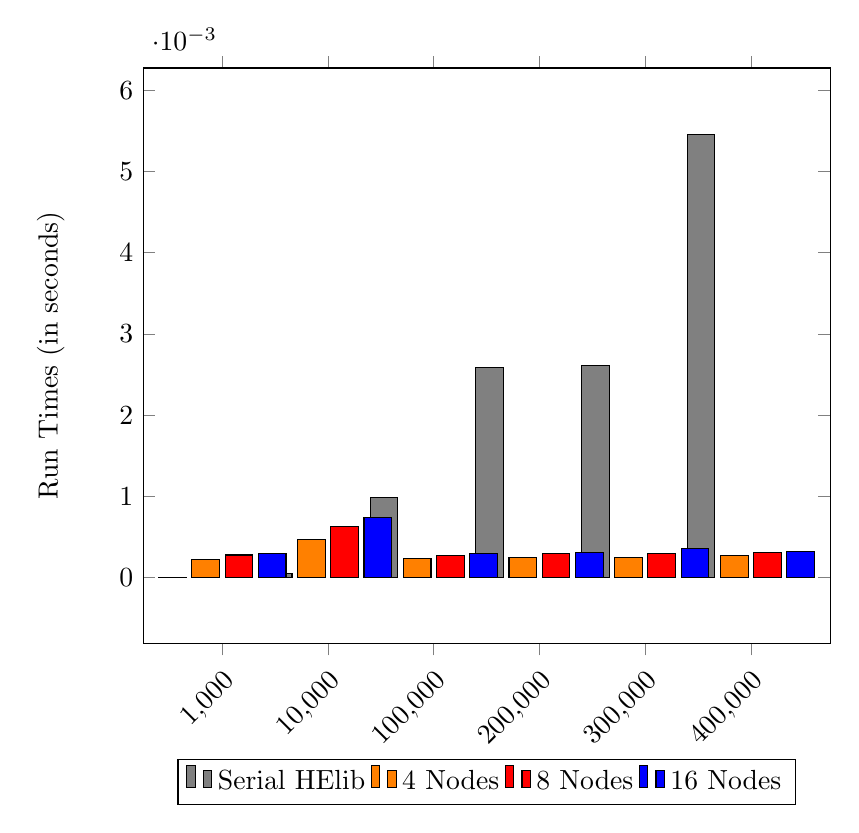
\begin{tikzpicture}

\begin{axis}[
    ybar,
    width=.85\textwidth,
    enlargelimits=0.15,
    legend style={at={(0.5,-0.2)},anchor=north,legend columns=-1},
    ylabel=Run Times (in seconds),
    symbolic x coords={$1{,}000$,$10{,}000$,$100{,}000$,$200{,}000$,$300{,}000$,$400{,}000$},
    xtick=data,
    x tick label style={rotate=45,anchor=north east},
    y label style={at={(axis description cs:-0.1,0.5)}, anchor=south},
]

\addplot[fill=gray]
    coordinates {
    ($1{,}000$,5.000E-06)($10{,}000$,4.800E-05)($100{,}000$,9.873E-04)($200{,}000$,2.588E-03)($300{,}000$,2.611E-03)($400{,}000$,5.457E-03) };
    
\addplot[fill=orange]
    coordinates {
    ($1{,}000$,2.240E-04)($10{,}000$,4.638E-04)($100{,}000$,2.373E-04)($200{,}000$,2.500E-04)($300{,}000$,2.438E-04)($400{,}000$,2.698E-04) };
    
\addplot[fill=red]
    coordinates {
    ($1{,}000$,2.773E-04)($10{,}000$,6.288E-04)($100{,}000$,2.740E-04)($200{,}000$,2.978E-04)($300{,}000$,2.913E-04)($400{,}000$,3.055E-04) };
    
\addplot[fill=blue]
    coordinates {
    ($1{,}000$,2.985E-04)($10{,}000$,7.418E-04)($100{,}000$,2.923E-04)($200{,}000$,3.083E-04)($300{,}000$,3.515E-04)($400{,}000$,3.235E-04) };
    
\legend{Serial HElib,4 Nodes,8 Nodes, 16 Nodes}
\end{axis}
\end{tikzpicture}

\caption{Add Third Level Run Times Comparison - Distribute}
\label{fig:level3ComparisonSerialDistributeAddVecs1}
\end{figure}

\begin{figure}[p]
\centering
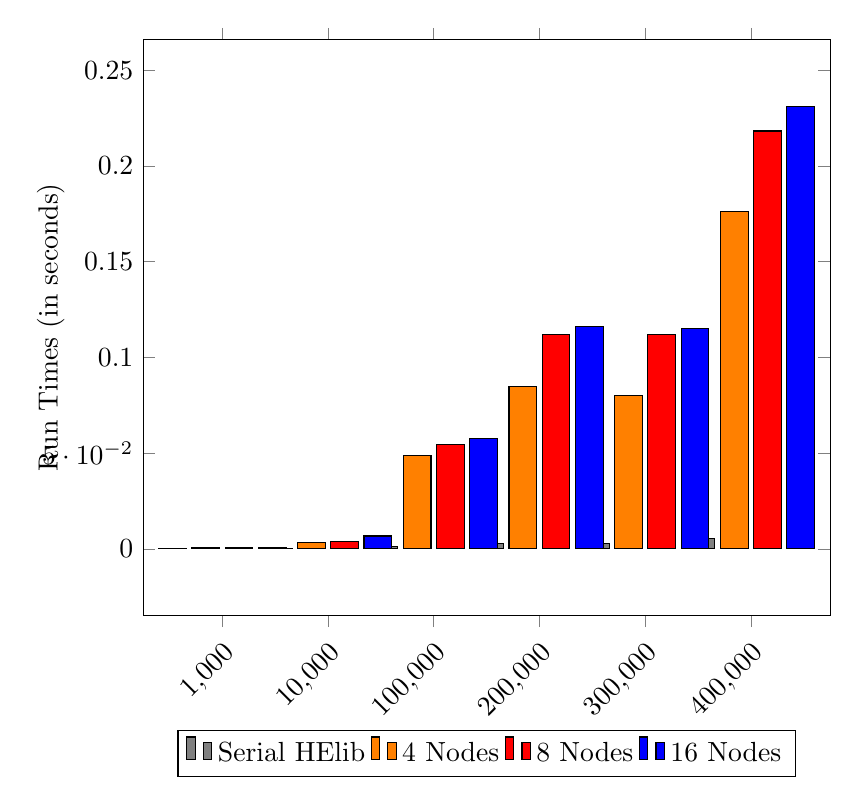
\begin{tikzpicture}

\begin{axis}[
    ybar,
    width=.85\textwidth,
    enlargelimits=0.15,
    legend style={at={(0.5,-0.2)},anchor=north,legend columns=-1},
    ylabel=Run Times (in seconds),
    symbolic x coords={$1{,}000$,$10{,}000$,$100{,}000$,$200{,}000$,$300{,}000$,$400{,}000$},
    xtick=data,
    x tick label style={rotate=45,anchor=north east},
    y label style={at={(axis description cs:-0.1,0.5)}, anchor=south},
]

\addplot[fill=gray]
    coordinates {
    ($1{,}000$,5.000E-06)($10{,}000$,4.800E-05)($100{,}000$,9.873E-04)($200{,}000$,2.588E-03)($300{,}000$,2.611E-03)($400{,}000$,5.457E-03) };
    
\addplot[fill=orange]
    coordinates {
    ($1{,}000$,5.158E-04)($10{,}000$,3.137E-03)($100{,}000$,4.874E-02)($200{,}000$,8.478E-02)($300{,}000$,8.023E-02)($400{,}000$,1.761E-01) };
    
\addplot[fill=red]
    coordinates {
    ($1{,}000$,5.903E-04)($10{,}000$,3.796E-03)($100{,}000$,5.461E-02)($200{,}000$,1.121E-01)($300{,}000$,1.122E-01)($400{,}000$,2.183E-01) };
    
\addplot[fill=blue]
    coordinates {
    ($1{,}000$,6.178E-04)($10{,}000$,6.692E-03)($100{,}000$,5.765E-02)($200{,}000$,1.163E-01)($300{,}000$,1.149E-01)($400{,}000$,2.313E-01) };
    
\legend{Serial HElib,4 Nodes, 8 Nodes, 16 Nodes}
\end{axis}
\end{tikzpicture}

\caption{Add Third Level Run Times Comparison - Sync}
\label{fig:level3ComparisonSerialDistributeAddVecs2}
\end{figure}

\begin{figure}[p]
\centering
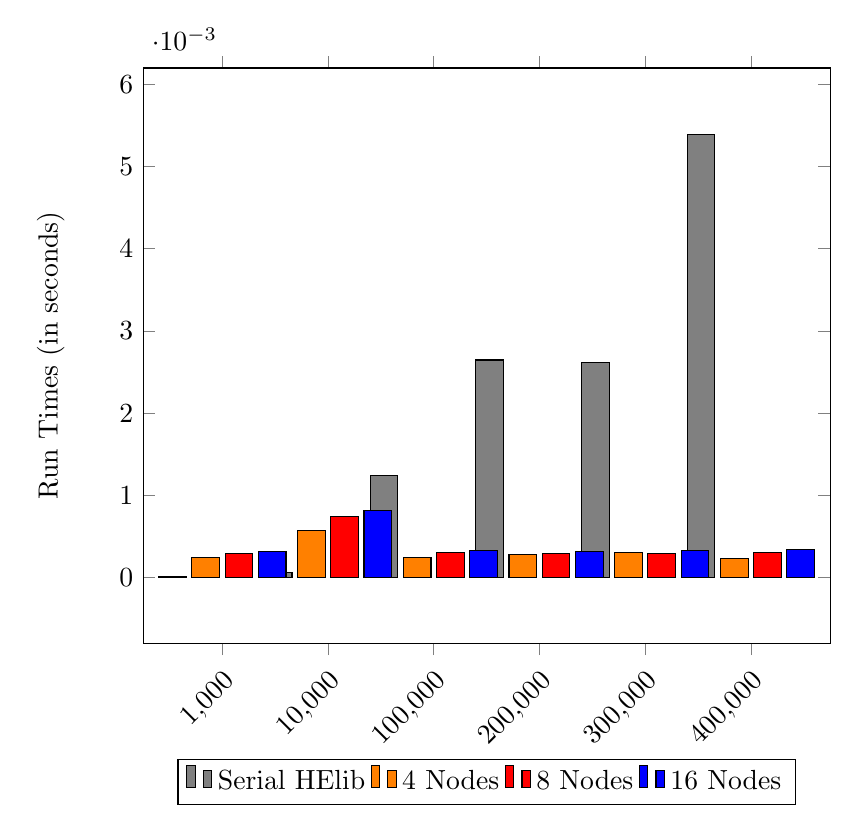
\begin{tikzpicture}

\begin{axis}[
    ybar,
    width=.85\textwidth,
    enlargelimits=0.15,
    legend style={at={(0.5,-0.2)},anchor=north,legend columns=-1},
    ylabel=Run Times (in seconds),
    symbolic x coords={$1{,}000$,$10{,}000$,$100{,}000$,$200{,}000$,$300{,}000$,$400{,}000$},
    xtick=data,
    x tick label style={rotate=45,anchor=north east},
    y label style={at={(axis description cs:-0.1,0.5)}, anchor=south},
]

\addplot[fill=gray]
    coordinates {
    ($1{,}000$,5.000E-06)($10{,}000$,5.850E-05)($100{,}000$,1.238E-03)($200{,}000$,2.646E-03)($300{,}000$,2.614E-03)($400{,}000$,5.391E-03) };
    
\addplot[fill=orange]
    coordinates {
    ($1{,}000$,2.405E-04)($10{,}000$,5.700E-04)($100{,}000$,2.470E-04)($200{,}000$,2.760E-04)($300{,}000$,2.995E-04)($400{,}000$,2.340E-04) };
    
\addplot[fill=red]
    coordinates {
    ($1{,}000$,2.915E-04)($10{,}000$,7.465E-04)($100{,}000$,3.015E-04)($200{,}000$,2.950E-04)($300{,}000$,2.955E-04)($400{,}000$,3.085E-04) };
    
\addplot[fill=blue]
    coordinates {
    ($1{,}000$,3.130E-04)($10{,}000$,8.175E-04)($100{,}000$,3.270E-04)($200{,}000$,3.190E-04)($300{,}000$,3.270E-04)($400{,}000$,3.445E-04) };
    
\legend{Serial HElib,4 Nodes,8 Nodes, 16 Nodes}
\end{axis}
\end{tikzpicture}

\caption{Sub Third Level Run Times Comparison - Distribute}
\label{fig:level3ComparisonSerialDistributeSubVecs1}
\end{figure}

\begin{figure}[p]
\centering
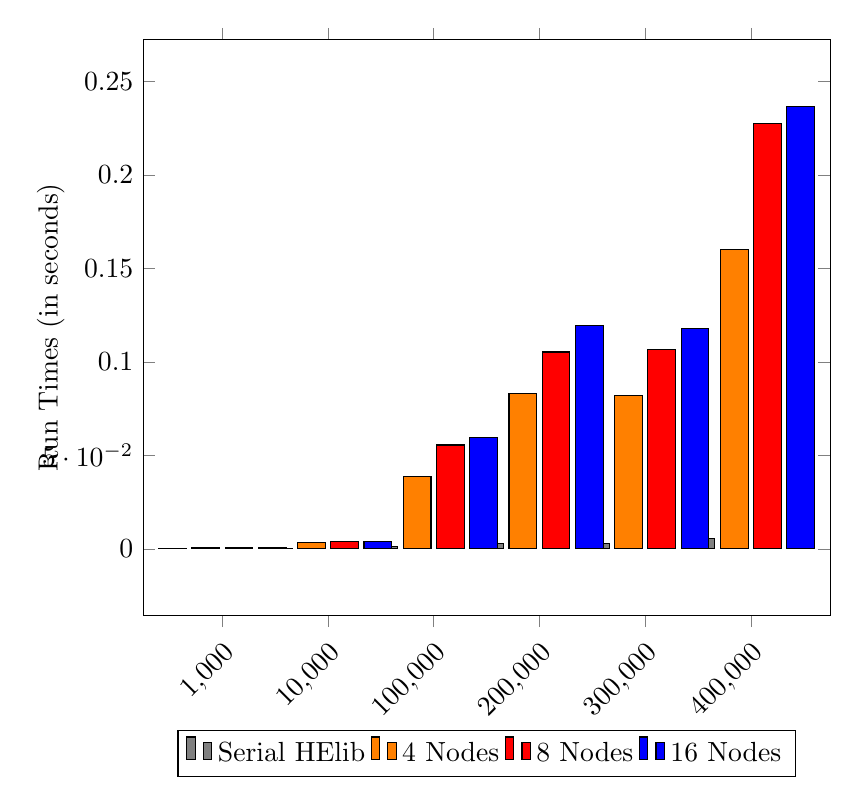
\begin{tikzpicture}

\begin{axis}[
    ybar,
    width=.85\textwidth,
    enlargelimits=0.15,
    legend style={at={(0.5,-0.2)},anchor=north,legend columns=-1},
    ylabel=Run Times (in seconds),
    symbolic x coords={$1{,}000$,$10{,}000$,$100{,}000$,$200{,}000$,$300{,}000$,$400{,}000$},
    xtick=data,
    x tick label style={rotate=45,anchor=north east},
    y label style={at={(axis description cs:-0.1,0.5)}, anchor=south},
]

\addplot[fill=gray]
    coordinates {
    ($1{,}000$,5.000E-06)($10{,}000$,5.850E-05)($100{,}000$,1.238E-03)($200{,}000$,2.646E-03)($300{,}000$,2.614E-03)($400{,}000$,5.391E-03) };
    
\addplot[fill=orange]
    coordinates {
    ($1{,}000$,5.260E-04)($10{,}000$,3.162E-03)($100{,}000$,3.861E-02)($200{,}000$,8.301E-02)($300{,}000$,8.203E-02)($400{,}000$,1.599E-01) };
    
\addplot[fill=red]
    coordinates {
    ($1{,}000$,5.940E-04)($10{,}000$,3.855E-03)($100{,}000$,5.553E-02)($200{,}000$,1.053E-01)($300{,}000$,1.066E-01)($400{,}000$,2.277E-01) };
    
\addplot[fill=blue]
    coordinates {
    ($1{,}000$,6.060E-04)($10{,}000$,4.045E-03)($100{,}000$,5.938E-02)($200{,}000$,1.196E-01)($300{,}000$,1.178E-01)($400{,}000$,2.368E-01) };
    
\legend{Serial HElib,4 Nodes, 8 Nodes, 16 Nodes}
\end{axis}
\end{tikzpicture}

\caption{Sub Third Level Run Times Comparison - Sync}
\label{fig:level3ComparisonSerialDistributeSubVecs2}
\end{figure}

\begin{figure}[p]
\centering
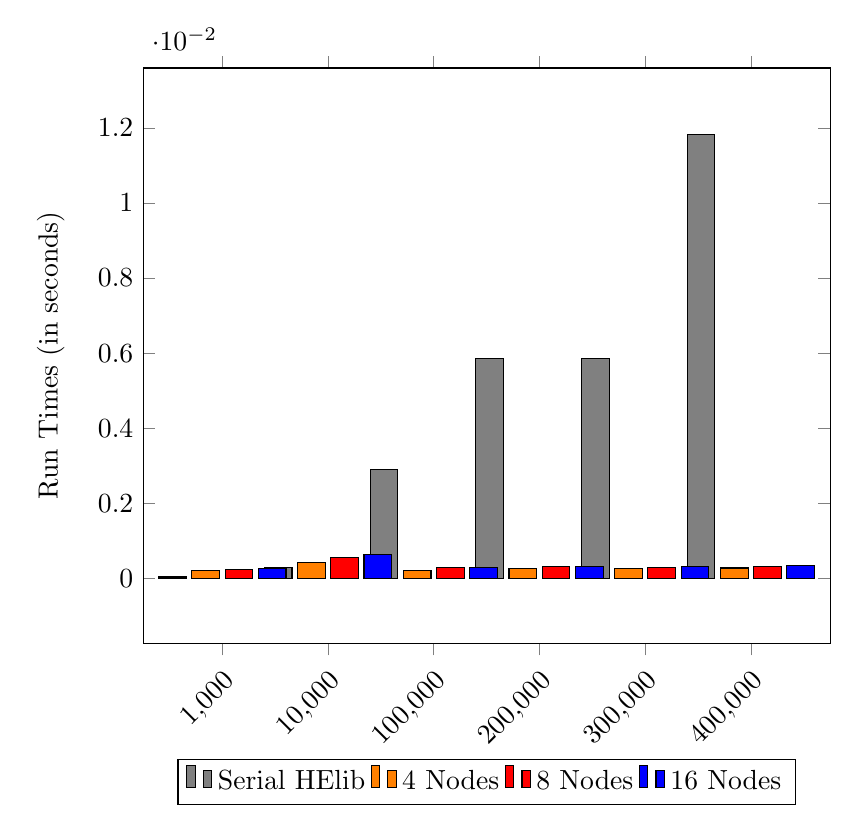
\begin{tikzpicture}

\begin{axis}[
    ybar,
    width=.85\textwidth,
    enlargelimits=0.15,
    legend style={at={(0.5,-0.2)},anchor=north,legend columns=-1},
    ylabel=Run Times (in seconds),
    symbolic x coords={$1{,}000$,$10{,}000$,$100{,}000$,$200{,}000$,$300{,}000$,$400{,}000$},
    xtick=data,
    x tick label style={rotate=45,anchor=north east},
    y label style={at={(axis description cs:-0.1,0.5)}, anchor=south},
]

\addplot[fill=gray]
    coordinates {
    ($1{,}000$,2.967E-05)($10{,}000$,2.838E-04)($100{,}000$,2.887E-03)($200{,}000$,5.845E-03)($300{,}000$,5.850E-03)($400{,}000$,1.183E-02) };
    
\addplot[fill=orange]
    coordinates {
    ($1{,}000$,2.015E-04)($10{,}000$,4.190E-04)($100{,}000$,2.150E-04)($200{,}000$,2.585E-04)($300{,}000$,2.668E-04)($400{,}000$,2.700E-04) };
    
\addplot[fill=red]
    coordinates {
    ($1{,}000$,2.427E-04)($10{,}000$,5.405E-04)($100{,}000$,2.872E-04)($200{,}000$,3.077E-04)($300{,}000$,2.953E-04)($400{,}000$,3.198E-04) };
    
\addplot[fill=blue]
    coordinates {
    ($1{,}000$,2.548E-04)($10{,}000$,6.265E-04)($100{,}000$,2.853E-04)($200{,}000$,3.130E-04)($300{,}000$,3.157E-04)($400{,}000$,3.338E-04) };
    
\legend{Serial HElib,4 Nodes,8 Nodes, 16 Nodes}
\end{axis}
\end{tikzpicture}

\caption{Mul Third Level Run Times Comparison - Distribute}
\label{fig:level3ComparisonSerialDistributeMulVecs1}
\end{figure}

\begin{figure}[p]
\centering
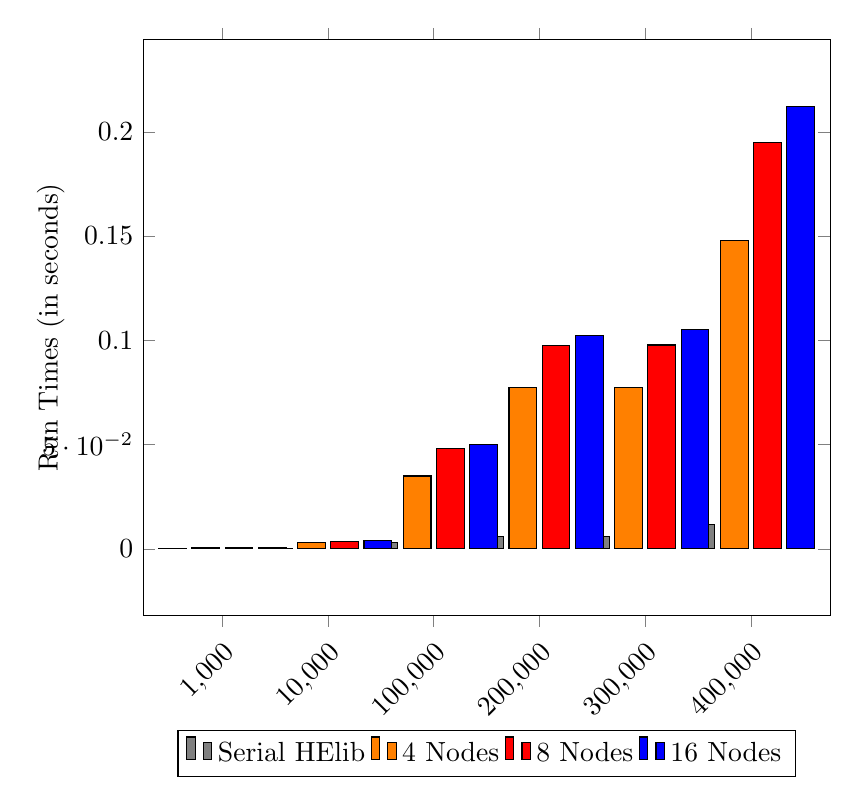
\begin{tikzpicture}

\begin{axis}[
    ybar,
    width=.85\textwidth,
    enlargelimits=0.15,
    legend style={at={(0.5,-0.2)},anchor=north,legend columns=-1},
    ylabel=Run Times (in seconds),
    symbolic x coords={$1{,}000$,$10{,}000$,$100{,}000$,$200{,}000$,$300{,}000$,$400{,}000$},
    xtick=data,
    x tick label style={rotate=45,anchor=north east},
    y label style={at={(axis description cs:-0.1,0.5)}, anchor=south},
]

\addplot[fill=gray]
    coordinates {
    ($1{,}000$,2.967E-05)($10{,}000$,2.838E-04)($100{,}000$,2.887E-03)($200{,}000$,5.845E-03)($300{,}000$,5.850E-03)($400{,}000$,1.183E-02) };
    
\addplot[fill=orange]
    coordinates {
    ($1{,}000$,5.110E-04)($10{,}000$,2.875E-03)($100{,}000$,3.495E-02)($200{,}000$,7.733E-02)($300{,}000$,7.744E-02)($400{,}000$,1.479E-01) };
    
\addplot[fill=red]
    coordinates {
    ($1{,}000$,5.608E-04)($10{,}000$,3.490E-03)($100{,}000$,4.801E-02)($200{,}000$,9.767E-02)($300{,}000$,9.774E-02)($400{,}000$,1.948E-01) };
    
\addplot[fill=blue]
    coordinates {
    ($1{,}000$,5.807E-04)($10{,}000$,3.869E-03)($100{,}000$,5.007E-02)($200{,}000$,1.022E-01)($300{,}000$,1.051E-01)($400{,}000$,2.123E-01) };
    
\legend{Serial HElib,4 Nodes, 8 Nodes, 16 Nodes}
\end{axis}
\end{tikzpicture}

\caption{Mul Third Level Run Times Comparison - Sync}
\label{fig:level3ComparisonSerialDistributeMulVecs2}
\end{figure}

Table \ref{tab:DistributedLevel3RuntimesDistribute4Nodes}, Table \ref{tab:DistributedLevel3RuntimesDistribute8Nodes}, and Table \ref{tab:DistributedLevel3RuntimesDistribute16Nodes} display the distribute run times for each operation across the three cluster sizes. Table \ref{tab:DistributedLevel3RuntimesSync4Nodes}, Table \ref{tab:DistributedLevel3RuntimesSync8Nodes}, and Table \ref{tab:DistributedLevel3RuntimesSync16Nodes} display the sync run times for each operation across the three cluster sizes. These times have been split into two plots for each operation. One group of plots focuses on the distribute times (the time it took to partition the data and assign the work) and compares them to the overall run time of the serial version. These are the \say{Distribute} plots, Figure \ref{fig:level3ComparisonSerialDistributeAddVecs1}, Figure \ref{fig:level3ComparisonSerialDistributeSubVecs1}, and Figure \ref{fig:level3ComparisonSerialDistributeMulVecs1}. The second group of plots display the sync time (the time the compute nodes took to receive the data, compute the results, and send the data back to the dispatcher node) compared to the overall run time for the serial design. Figure \ref{fig:level3ComparisonSerialDistributeAddVecs2}, Figure \ref{fig:level3ComparisonSerialDistributeSubVecs2}, and Figure \ref{fig:level3ComparisonSerialDistributeMulVecs2} display these results, and are the \say{Sync} plots.

By looking at the \say{Distribute} plots, one can see that the partitioning of data and assignment of work times across all clusters sizes and operations remains constant even when the input sizes are increased. This looks good, but remember that this part of the work only records the times it takes to partition the data and assign the work, not send the data to the compute nodes. Only non-blocking sends and receives are scheduled during this portion of the recording. The actual sending and receiving between the dispatcher and compute nodes happens mostly during the sync portion of the recording. This is because the non-blocking send and receive functions only schedule requests, which are later fulfilled in the background, during the sync part. So it is to be expected that these results are seen.

The \say{Sync} plots show where this design is failing. The amount of time needed to send the data over the network to the compute nodes, have them perform the operation and then send the data back is much greater than the serial times. This has to do with the network speed, which causes a bottleneck, and which is responsible for the plateau characteristic seen in the circuit and function level times. The network speeds are much too slow in this environment to allow for this design to be viable. With better speeds (ones which would not cause this bottleneck to happen) this design might provide better results. Additionally, future work to try and minimize the amount of data transfers between the dispatcher and compute nodes could also lead to better run times.

\section{Evaluation Conclusions} \label{sec:EvaluationConclusions}
As mentioned in the introduction of this chapter, when working with distributed systems, the overhead time, which comes from the memory transfer phases of each design, usually is the downfall of distributed systems. The same is true for these designs. GPUHElib suffered from slow transfer times between the CPU and GPU, which caused slow downs compared to the serial version. Similarly, DistributedHElib suffered from slow network speeds, which caused a bottleneck when transferring data between the dispatcher node and the compute nodes. With better transfer speeds, both of these designs might be viable, however under these circumstances, they are not.